% report.tex : Main file for the LaTeX report.
\documentclass{report}[14pt]

\usepackage{amsmath}
\usepackage{graphicx,color,geometry}
\usepackage{subcaption}
\usepackage{hyperref}
\usepackage{amsfonts}

\newtheorem{definition}{Definition}[section]
\newtheorem{lemma}{Lemma}[section]
\newtheorem{proposition}{Proposition}[section]
\newtheorem{example}{Example}[section]
\newtheorem{theorem}{Theorem}[section]

\begin{document}
	\begin{titlepage}
		\begin{center}
			\vspace*{1cm}
			\Large { A Report}

			\vspace{0.5cm}

			\Large{on}

			\vspace{0.5cm}
			\LARGE { \textbf{Shape from Shading - Theory and Applications} }

			\vspace{2cm}

			\Large{By}

			\vspace{1cm}

			\LARGE{\emph{Balaje K \\ Sanath Keshav}}

			\vspace{3cm}
			\LARGE{ \textbf{Tata Institute of Fundamental Research - Center for Applicable Mathematics}}\\

			\vspace{0.5cm}
			
\includegraphics[scale = 1]{Images/TIFR_logo.png}

			\vspace{0.5cm}
			July 2016
		\end{center}
	\end{titlepage}

	\chapter*{Acknowledgements}
	We would like to sincerely thank Prof. G.D.Veerappa Gowda for providing us with an opportunity to work at TIFR-CAM on this project. We thank Dr. Aekta Aggarwal for providing us with valuable inputs, suggestions and tips throughout the Internship. \\
	
	\noindent
	We thank our parents for providing us with constant support and encouragement which helped us throughout this project. We thank the Almighty, without which none of this would have been possible.\\
	
	\noindent
	Once again we thank them all.

	\listoffigures
	\tableofcontents
	\chapter{Introduction}
	% chapters/intro.tex 
%	First chapter in VSRP Report.

Shape from Shading (SfS) is a 3D image reconstruction technique, in which the shape of a 3D object (output) is retrieved from a 2D image (input). The 2D image is a light intensity map of the 3D object, which is a grayscale image. The intensity map is obtained by flashing light over the object from a particular point (known \textit{apriori}) to illuminate the object. Then a mathematical model is constructed to relate the pixel intensity in the input image to obtain the depth information of the 3D surface. Figure (\ref{fig:1}) gives a flow chart of the process in SfS.

\begin{figure}[h!]
	\centering
	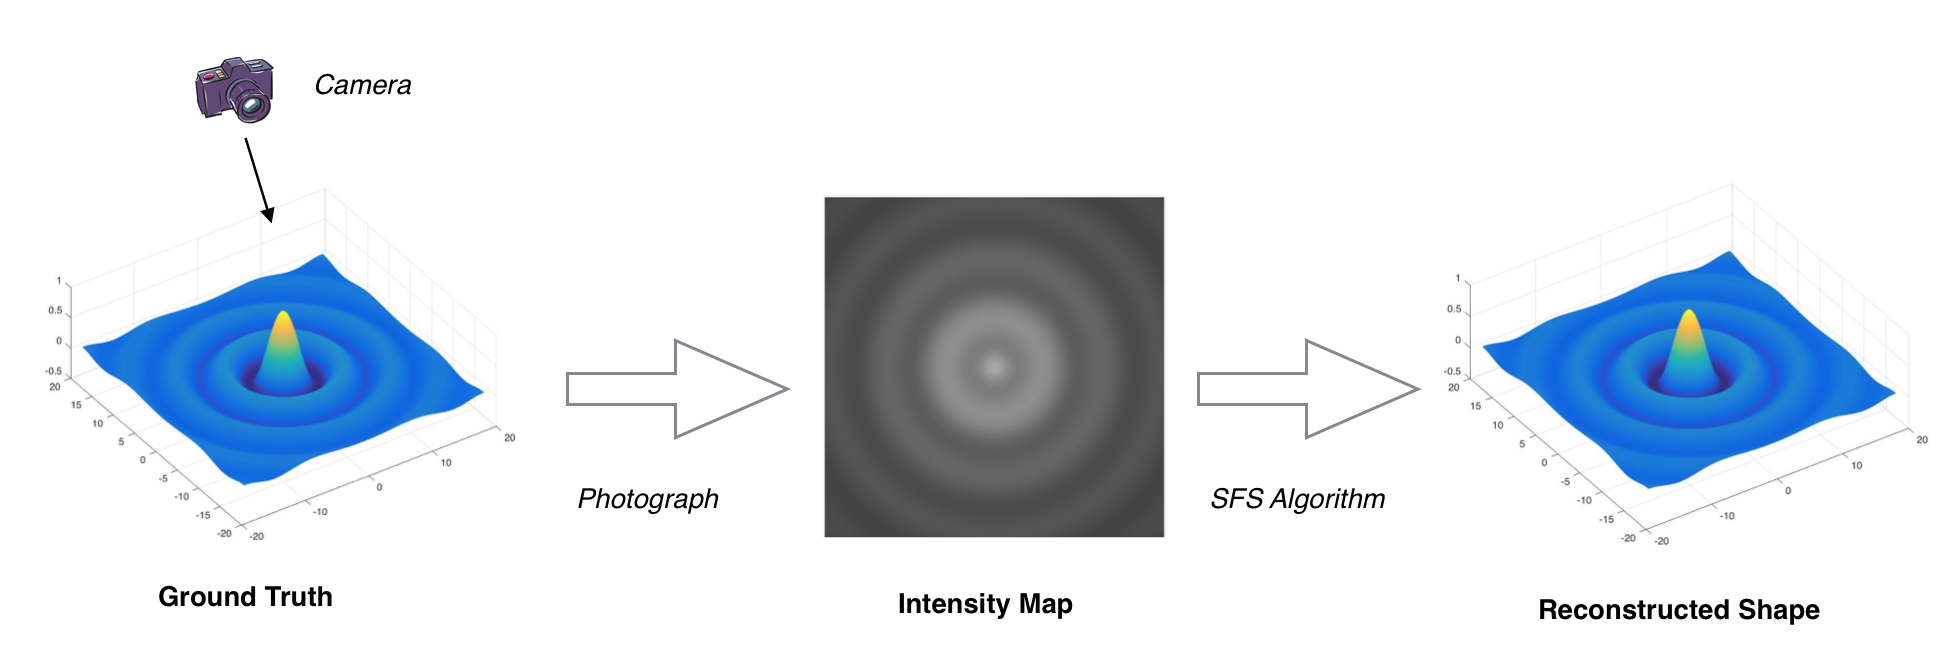
\includegraphics[width = 15.5cm]{images/flow.png}
	\caption{\textbf{Shape from Shading :} The \emph{ground truth} is the original object and SfS attempts to reconstruct it, just from knowing the \textit{Intensity map}}
	\label{fig:1}
\end{figure}

\noindent
The relation between the intensity of a pixel and the height of our reconstructed surface is given by a PDE. K.P.Horn\cite{horn} has given an eikonal equation type approach to formulate the Shape from Shading problem. This is known as the \textbf{orthographic projection model}. Rouy and Tourin\cite{rouy} came up with a viscosity solution approach to the model, and constructed an upwind type numerical scheme to solve the Eikonal type equation. Though this model was simple and effective, it suffered from a disadvantage because of singular points (More on singular points will be discussed in the coming chapters), where uniqueness of the solution is lost.\\

\noindent
 Prados and Faugeras\cite{prados2} came up with a much more realistic model that takes care of this difficulty. To solve the resulting PDE, Prados and Faugeras\cite{prados1} formulates a minimization approach, although solving the PDE using numerical techniques works as good. In this work, we present a numerical method to solve the PDE that arises due to Prados's work without using the minimization approach. Some applications of shape from shading can be found in \cite{prados1}\\
 
 \noindent
 This report is divided into 6 chapters. Chapter 2 introduces the reader to Hamilton Jacobi Equations (HJE), which is the backbone of Shape from Shading. This chapter discusses the need for viscosity solutions, and some existence, uniqueness results. Chapter 3 deals with the development of Orthographic Projection Model and discusses the notion of singular points and some ways to overcome the problem. Chapter 4 discusses the Perspective Projection approach to SfS problems and presents some existence and uniqueness results. Chapter 5 deals with the construction of some numerical schemes to solve the Eikonal Equation in a variety of domains, using the immersed boundary method. Numerical schemes to solve the SfS problems are discussed and the stability of these schemes are explained. Chapter 6 presents the results of some numerical experiments that were conducted on a variety of synthetic images to illustrate SfS.


	\chapter{Viscosity Solutions to Hamilton Jacobi Equations}
	% chapters/mathbg.tex
%  Second chapter in mathbg.tex

\section{Hamilton Jacobi Equations}
A Hamilton Jacobi equation (HJE) is a non-linear Partial Differential Equation of the form
\begin{eqnarray}
  H(\mathbf{x},u(\mathbf{x}),Du(\mathbf{x})) &=& 0 \;\; \text{in} \;\; \Omega \label{eq:1}\\
  u(\mathbf{x}) &=& \varphi(\mathbf{x}) \;\; \text{on} \;\; \partial \Omega \label{eq:2}
\end{eqnarray}
where $\mathbf{x} = (x_1,\dots,x_n) \in \mathbb{R}^n$, $u(\mathbf{x}) \in \mathbb{R}$ and $Du(\mathbf{x})$ is the first order derivative of u in $\mathbb{R}^n$, defined by,
\begin{equation}
  Du(\mathbf{x}) = \left(\frac{\partial u}{\partial x_1},\dots ,\frac{\partial u}{\partial x_n}\right)^T
\end{equation}

\noindent
The function $H(\mathbf{x},u(\mathbf{x}),Du(\mathbf{x})) : \Omega \times \mathbb{R} \times \mathbb{R}^n \to \mathbb{R}$ is known as the Hamiltonian. $u(\mathbf{x})$ is our unknown function. The problem defined by (\ref{eq:1})-(\ref{eq:2}) is known as the Dirichlet Boundary Value Problem (BVP). The other class of problem, known as the Cauchy Problem is given by,
\begin{eqnarray}
  \frac{\partial u }{\partial t} + H(\mathbf{x},t,u(\mathbf{x},t),Du(\mathbf{x},t)) &=& 0 \qquad \qquad \; \text{in} \;\; \Omega \times ]0,T] \label{eq:3}\\
  u(\mathbf{x},t) &=& \varphi(\mathbf{x},t) \qquad \text{on} \;\; \partial \Omega \times ]0,T]\label{eq:4}\\
  u(\mathbf{x},0) &=& u_0(\mathbf{x}) \qquad \;\; \text{in} \;\; \Omega
\end{eqnarray}

\noindent
The function $u_0(\mathbf{x})$ is known as the initial condition. These types of PDEs were investigated by the Irish Mathematician William Rowan Hamilton\cite{ham1,ham2}.

\section{Well Posedness}
According to Hadamard\cite{hadamard}, a mathematical model has to be well posed. A well posed problem has the following properties,
\begin{enumerate}
\item
\textbf{Existence} - There exists a solution to the problem.
\item
\textbf{Uniqueness} - There exists atmost one solution to the problem.
\item
\textbf{Stability} - The solution depends continuously on the data.
\end{enumerate}

\noindent
The existence of a solution to the HJE can be assured if we enlarge the space of functions under consideration. For example, as we will see soon enough, the Eikonal Equation has a solution in $C^0$, the space of continuous functions, but not in $C^1$, the space of continuously differentiable functions. The uniqueness of a problem is normally obtained by supplying additional information like initial/boundary data, so that we can capture the physically relevant solution. Stability is an important criterion while constructing the numerical schemes, as a small perturbation in the initial data should produce small changes in the solution to the PDE. This situation becomes relevant when we tend the mesh size $h \to 0$, the computed solution should converge to the exact solution of the PDE\cite{lax}.

\section{Viscosity Solutions}
\subsection{Need for Viscosity Solutions}
The Hamilton Jacobi Equations are normally not well-posed under the classical solution approach. The properties of existence and uniqueness in the classical sense are no longer satisfied.\\

\noindent
For example, when we consider solving the Eikonal Equation in 1D,
\begin{eqnarray}
  \lvert u' \rvert &=& 1 \qquad \text{in} \;\;\; \Omega \equiv (0,1)\label{eq:5}\\
  u &=& 0 \qquad \text{on} \;\;\; \partial \Omega \equiv \{0,1\}\label{eq:6}
\end{eqnarray}
which is a HJE, it can be shown that the solution to the problem does not exist in $C^1$. This can be easily proved using contradiction. Consider that we are looking for a solution $u \in C^1$. As we have, $u(0) = u(1) = 0$, by Rolle's Theorem, $\exists x_0 \in (0,1)$ such that $u'(x_0) = 0$, which contradicts (\ref{eq:5}). So $u \notin C^1$. This shows that, we have solutions that are not differentiable at certain points on the domain but $u \in C^0$. Such solutions satisfy the PDE in a ``weaker" sense and hence are called \textbf{weak solutions}.\\

\noindent
One can see that $u^+(x) = \frac{1}{2} - \left\lvert \frac{1}{2} - x\right\rvert$ is a \textit{weak} solution to the Dirichlet Problem (\ref{eq:5})-(\ref{eq:6}). But we can see that $u^-(x) = -u^+(x)$ is a solution to the problem as well. Hence, the classical approach becomes insufficient to guarantee a unique solution to the Dirichlet Problem.\\

\noindent
\subsection{Viscosity Solutions}
P.L.Lions and M.G.Crandall\cite{lions} came up with a setting to obtain the
existence and uniqueness properties for the Hamilton Jacobi
Equation. They are known as \textbf{viscosity solutions}. The term
\textbf{viscosity} is used because solution to the HJE is obtained by
adding a viscosity term $\epsilon u_{xx}$ to the HJE and letting
$\epsilon \to 0$ to obtain the solution to our original PDE. Before we
see how to obtain the viscosity solutions, we must find a way to deal
with the non-differentiable points in $C^0$ solutions. For this we
define \textbf{super differentials} and \textbf{sub
  differentials}. Super- and sub-differentials replaces the classical
derivatives at non-differentiable points in the functions and are
equivalent to the classical definition at differentiable points.

\noindent
For the following HJE,
\begin{eqnarray}
  H(\mathbf{x},\nabla u(\mathbf{x})) &=& 0 \qquad \text{in} \;\;\; \Omega\\
  u(\mathbf{x}) &=& \varphi(\mathbf{x}) \qquad \text{on} \;\;\; \partial \Omega
\end{eqnarray}
\begin{definition}
  A continuous function $u\in C^0$ is a viscosity solution to the HJE,
  if it satisfies the following conditions
  \begin{enumerate}
  \item \textbf{Viscosity Subsolution} : For any test function
    $\varphi \in C^1$, if $\mathbf{x_o}$ is the local maximum of
    $u-\varphi$, then
    \begin{equation}\nonumber
      H(\mathbf{x_o}, \nabla u(\mathbf{x_o}) ) \le 0
    \end{equation}

  \item \textbf{Viscosity Supersolution} : For any test function
    $\varphi \in C^1$, if $\mathbf{x_o}$ is the local minimum of
    $u-\varphi$, then
    \begin{equation}\nonumber
      H(\mathbf{x_o}, \nabla u(\mathbf{x_o}) ) \ge 0
    \end{equation}
  \end{enumerate}
  \label{def:1}
\end{definition}
An alternate, but an equivalent definition of the same is given using
sub- and super- differentials.
\begin{definition}
  A continuous function $u\in C^0$ is a viscosity solution to the HJE,
  if it satisfies the following conditions
  \begin{enumerate}
  \item \textbf{Viscosity Subsolution} : $H(\mathbf{x},p) \le 0$ for
    all $\mathbf{x} \in \mathbb{R}^n$ and $p\in D^+u$

  \item \textbf{Viscosity Supersolution} : $H(\mathbf{x},q) \ge 0$ for
    all $\mathbf{x} \in \mathbb{R}^n$ and $q\in D^-u$
  \end{enumerate}
  \label{def:2}
  where,
  \begin{eqnarray}
    D^+u &=& \left\{p \in \mathbb{R}^n \;\; \Big |\;\; \limsup\limits_{y\to x} \frac{u(y)-u(x) - p.(y-x)}{\lvert y-x \rvert} \le 0\right\}\label{eq:7}\\
    D^-u &=& \left\{q \in \mathbb{R}^n \;\; \Big |\;\; \liminf\limits_{y\to x} \frac{u(y)-u(x) - q.(y-x)}{\lvert y-x \rvert} \ge 0\right\}\label{eq:8}
  \end{eqnarray}
\end{definition}

\noindent
The sets $D^+u$ and $D^-u$ are known as the super- and
sub-differentials, respectively. A collection of some properties of
sub- and super-differentials are listed below. Refer \cite{yong} for more
details.
\begin{enumerate}
\item $D^+u$ and $D^-u$ are convex subsets of $\mathbb{R}^n$.
\item If $u$ is differentiable at any point $\mathbf{x}$, then
  \begin{equation}\nonumber
    \{Du(\mathbf{x})\} = D^+u(\mathbf{x}) = D^-u(\mathbf{x})
  \end{equation}
\item If for some $\mathbf{x}$, both $D^+u$ and $D^-u$ are non-empty,
  \begin{equation}\nonumber
    \{Du(\mathbf{x})\} = D^+u(\mathbf{x}) = D^-u(\mathbf{x})
  \end{equation}
\item
  $D^+(\alpha u)(\mathbf{x}) = \alpha D^+u(\mathbf{x}), \quad \alpha >
  0$
\item
  $D^+(\alpha u)(\mathbf{x}) = \alpha D^-u(\mathbf{x}), \quad \alpha <
  0$
\item
  $D^+(u+\varphi)(\mathbf{x}) = D^+u(\mathbf{x}) +
  D\varphi(\mathbf{x}), \quad \text{if} \;\varphi \in C^1$
\item
  $D^+u_\alpha(\mathbf{x}) = \alpha D^+u(\mathbf{x}) +
  (1-\alpha)D\varphi\nonumber$ \hspace{5mm} \text{where,}
  $\quad u_\alpha = \alpha u(\mathbf{x}) +
  (1-\alpha)\varphi(\mathbf{x)}\nonumber$
\end{enumerate}

\noindent
The following example illustrates the procedure for calculating the
super and sub-differentials of a function in 1D. We do this for
$u^+(x) = 1 - \lvert x \rvert$ and use them to isolate the viscosity
solution of the following Eikonal equation with Dirichlet boundary
data. (In fact we show that $u^+(x)$ is the viscosity solution to our
Dirichlet BVP).
\begin{eqnarray}
  |u'| &=& 1 \qquad \text{in} \;\; \Omega \equiv (-1,1)\\
  u &=& 0 \qquad \text {on} \;\; \partial \Omega \equiv \{-1,1\}
\end{eqnarray}
\begin{example}
  Super and sub differential of $u(x) = 1-\lvert x \rvert$\\

  \noindent
  \textbf{Super Differential} $D^+u$:\\

  \noindent
  We consider the case only when $x=0$, as $x=0$ is the only
  non-differentiable point. The classical definition of the derivative
  holds for the case $x\ne 0$ as the function is differentiable at
  these points. For full details, refer \cite{yong}
  \begin{enumerate}
  \item $x = 0$
    \begin{itemize}
    \item
      $y \ge 0 \implies \lvert y \rvert = y \implies 1 - \lvert y
      \rvert = 1 - y$
      \begin{eqnarray}
        &\iff&\limsup \limits_{y \to x} \frac{u(y)-u(x) - p(y-x)}{\lvert y -x \rvert} \le 0\\
        &\iff& \limsup \limits_{y \to 0} \frac{(1-y)-1 - p(y-0)}{\lvert y -0 \rvert} \le 0\\
        &\iff& \limsup \limits_{y \to 0} \frac{-y - py}{ y } \le 0\\
        \text{As} \quad y \ge 0 &\iff& -y-py \le 0 \implies y(1+p) \ge 0 \nonumber
                                       \implies p \ge -1
      \end{eqnarray}

    \item
      $y \le 0 \implies \lvert y \rvert = -y \implies 1 - \lvert y
      \rvert = 1 + y$
      \begin{eqnarray}
        &\iff&\limsup \limits_{y \to x} \frac{u(y)-u(x) - p(y-x)}{\lvert y -x \rvert} \le 0\\
        &\iff& \limsup \limits_{y \to 0} \frac{(1+y)-1 - p(y-0)}{\lvert y -0 \rvert} \le 0\\
        &\iff& \limsup \limits_{y \to 0} \frac{y - py}{ -y } \le 0\\
        \text{As} \quad -y \ge 0 &\iff& y-py \le 0 \implies y(1-p) \le 0 \nonumber
                                        \implies p \le 1
      \end{eqnarray}
    \end{itemize}
    From the two cases, we conclude that when $x=0$, $p\in[-1,1]$

  \item $x < 0$, we have from the classical definition $p = \{1\}$

  \item $x > 0$, we have from the classical definition $p = \{-1\}$
  \end{enumerate}
  Hence from the above steps, we conclude that the super differential
  of $1-\lvert x \rvert$ is
  \begin{eqnarray}
    D^+u = \left\{
    \begin{array}{ll}
      1 & x \le 0\\
      \left[-1,1\right] & x = 0\\
      -1 & x\ge 0
    \end{array}
           \right.\label{eq:9}
  \end{eqnarray}

\noindent
Following the same procedure, we can find the sub-differential of $1-\lvert x \rvert$.\\

\noindent
\textbf{Sub Differential} $D^-u$
\begin{enumerate}
\item $x = 0$
  \begin{itemize}
  \item
    $y \ge 0 \implies \lvert y \rvert = y \implies 1 - \lvert y \rvert
    = 1 - y$
    \begin{eqnarray}
      &\iff&\liminf \limits_{y \to x} \frac{u(y)-u(x) - p(y-x)}{\lvert y -x \rvert} \ge 0\\
      &\iff& \liminf\limits_{y \to 0} \frac{(1-y)-1 - p(y-0)}{\lvert y -0 \rvert} \ge 0\\
      &\iff& \liminf \limits_{y \to 0} \frac{-y - py}{ y } \ge 0\\
      \text{As} \quad y \ge 0 &\iff& -y-py \ge 0 \implies y(1+p) \le 0 \nonumber
                                     \implies p \le -1
    \end{eqnarray}

  \item
    $y \le 0 \implies \lvert y \rvert = -y \implies 1 - \lvert y
    \rvert = 1 + y$
    \begin{eqnarray}
      &\iff&\liminf \limits_{y \to x} \frac{u(y)-u(x) - p(y-x)}{\lvert y -x \rvert} \ge 0\\
      &\iff& \liminf \limits_{y \to 0} \frac{(1+y)-1 - p(y-0)}{\lvert y -0 \rvert} \ge 0\\
      &\iff& \liminf \limits_{y \to 0} \frac{y - py}{ -y } \ge 0\\
      \text{As} \quad -y \ge 0 &\iff& y-py \ge 0 \implies y(1-p) \ge 0 \nonumber
                                      \implies p \ge 1
    \end{eqnarray}
  \end{itemize}
  From the two cases, we conclude that when $x=0$, $p = \phi$

\item $x < 0$, we have from the classical definition $p = \{1\}$

\item $x > 0$, we have from the classical definition $p = \{-1\}$
\end{enumerate}
Hence from the above steps, we conclude that the sub differential of
$1-\lvert x \rvert$ is
\begin{eqnarray}
  D^-u = \left\{
  \begin{array}{ll}
    1 & x \le 0\\
    \emptyset & x = 0\\
    -1 & x\ge 0
  \end{array}
         \right. \label{eq:10}
\end{eqnarray}
\end{example}

\noindent
With the super- and sub- differentials in our hand, we now see how
this can be used to pick out the unique viscosity solution of the
Eikonal equation. Let us consider $u(x) = 1-\vert x \rvert$ and the
convex Hamiltonian $H(x,p) = \lvert p \rvert - 1$ for the Eikonal
equation. Now we have from \ref{eq:9}
\begin{eqnarray}
  \lvert p \rvert \le 1 &\implies& \lvert p \rvert - 1 \le 0\quad \forall p \in D^+u\\
                        &\implies& H(x,p) = \lvert p \rvert - 1 \le 0 \quad \forall p \in D^+u
\end{eqnarray}
Thus, the viscosity sub-solution condition is satisfied. Since $D^-u = \emptyset$ for $x=0$, the super-solution condition is satisfied trivially. Thus $u(x) = 1-\lvert x \rvert$ is a\textbf{ viscosity solution} to the Eikonal equation with homogeneous Dirichlet boundary conditions.\\

\noindent
But on the other hand, $u(x) = \lvert x \rvert - 1$ is \textbf{not a
  viscosity solution} to the Eikonal Equation with the convex
Hamiltonian $H(x,p) = \lvert p \rvert - 1$, as the super-solution
condition $H(x,p) \ge 0$ is not satisfied by the sub-differential of
$\lvert x \rvert - 1$. But $u(x) = \lvert x \rvert - 1$ is the
viscosity solution to the Eikonal equation with non-convex Hamiltonian
$H(x,p) = 1 - \lvert p \rvert$ and $u(x) = 1 - \lvert x \rvert$ is
not. This shows that the viscosity solution is dependent on the nature
of Hamiltonian used and \textit{changing the Hamiltonian does not
  preserve the \textbf{Viscosity Solution}}.

\section{Legendre Transform}
A Legendre Transform is a peculiar transformation which connects the
Hamiltonian and Lagrangian approaches in physics. Legendre transform
can be viewed as a means to express information in an alternate and a
simpler way. Zia et. al. in their paper titled ``Making sense of the
Legendre Transform''\cite{ZIA} presented a way to see Legendre transform as a
powerful mathematical tool. They explain the origins of the Legendre
Transform and its applications to various problems in Physics. In this
report, we see how the Legendre Transform is defined in the classical
sense and to extend the same to the viscosity setting.

\subsection{Classical Definition}
In this section, we see how the Legendre Transform is defined in the
classical sense. We assume a differentiable function $f:\mathbb{R}^n :
\mathbb{R}$ and its
gradient $\nabla f \in \mathbb{R}^n$. Writing the gradient as a map
\begin{equation}
  \nabla : \mathbb{R} \to \mathbb{R}^n
\end{equation}
Now we have the composite mapping,
\begin{equation}
  \nabla f : \mathbb{R}^n \xrightarrow{f} \mathbb{R}
  \xrightarrow{\nabla} \mathbb{R}^n
\end{equation}

\noindent
Now we are interested in defining an inverse map $(\nabla f)^{-1}$ for the
above composite mapping. Now we need to find the value of $x$ that
satisfies $s = \nabla f(x)$. Let us call that $\nabla h$, so that
$x = \nabla h(s)$. The procedure for finding out $h$ is illustrated
below in 1D.
\begin{eqnarray}
  &\implies&\frac{df}{dx} = s \nonumber\\
  &\implies& df = sdx \nonumber\\
  &\implies& df = d(sx) - xds\nonumber\\
  &\implies& df - d(sx) = -xds\nonumber\\
  &\implies& d(sx - f) = xds\nonumber\\
  &\implies& \frac{d}{ds}(sx - f) = x
\end{eqnarray}

\noindent
From this we get $h(s) = sx(s) - f(x(s))$. This is defined as the
Legendre Transform of the function $f(x)$.
\begin{definition}
  \textbf{Classical Legendre Transform of f(x)}\\
  Let $x\in\mathbb{R}^n$ and $S \subset \mathbb{R}^n$, and $s \in
  S$. The mapping $h(s):S \to \mathbb{R}$,
  \begin{equation}
    h(s) = \langle x,s \rangle - f(x(s))
  \end{equation}
  is known as the Legendre Transform of $f(x)$.
\end{definition}
This definition assumes that the function $f(x)$ is
differentiable. In the next subsection we will see how to extend the
Legendre Transform to a non-differentiable function like $\lvert x
\rvert$. We will also see how the Legendre transform is used to define
the compatibility condition on the boundary data to guarantee the
existence of solution to HJE. Before we move on, an example to
calculate the Legendre Transform for a smooth function is described below.
\begin{example}
  \textbf{Legendre Transform of $f(x) = x^2$}\\
  First we compute the relation between $x$ and $s$.
  \begin{eqnarray}
    s = \frac{df}{dx} = 2x\\
    \implies x = \frac{s}{2}
  \end{eqnarray}
  Then we use the definition of the Legendre Transform to get,
  \begin{eqnarray}
    &h(s)& = \frac{s^2}{2}- \frac{s^2}{4} \\
    \implies &h(s)& = \frac{s^2}{4}
  \end{eqnarray}

\end{example}

\subsection{Generalized Legendre Transform}
The generalised Legendre Transform is defined for functions having
non-differentiable points. The mapping $x \to \nabla f(x)$ us replaced
by a set valued mapping $x \to \partial f(x)$, where $\partial f(x)$
is the sub-differential of $f(x)$. The formal definition of the
Legendre Transform is given by,
\begin{definition}
  \textbf{Generalised Legendre Transform}\\

  \noindent
  Assume a convex function $f(x)$, where $x \in \mathbb{R}^n$ and $f :
  \mathbb{R}^n \to \mathbb{R}$. The generalised Legendre Transform is
  a mapping defined by
  \begin{equation}
    f^*(s) = \sup_{x}\{\langle s,x \rangle\ - f(x)\;\; :\;\; x \in
    domain(f) \} \label{eq:11}
  \end{equation}
\end{definition}

\noindent
We now end this section by presenting an example to calculate the
Generalised Legendre Transform of a non-differentiable function $f(x)
= \lvert x \rvert$.
\begin{example}
  \textbf{Legendre Transform of $f(x) = \lvert x \rvert$}\\

  \noindent
  Using the definition of the Generalised Legendre Transform,
  \begin{eqnarray}
    f^*(s) &=& \sup_{x}\{sx - \lvert x \rvert\}\\
    &=& \sup_{x} \left\{
      \begin{array}{ll}
        sx - x & x > 0\\
        sx + x & x < 0
      \end{array}
                 \right.\\
    &=& \sup_{x} \left\{
      \begin{array}{ll}
        (s-1)x & x > 0\\
        (s+1)x & x < 0
      \end{array}
    \right.
  \end{eqnarray}
  With this for $f^*(x) < +\infty$, we get a condition that $\lvert s
  \rvert < 1$. Finally, we obtain the Legendre Transform of $f(x)$ to
  be,
  \begin{equation}
     f^*(s) = \left\{
      \begin{array}{ll}
        0 & \lvert s \rvert < 1\\
        +\infty & \text{otherwise}
      \end{array}
    \right.
  \end{equation}
\end{example}

\section{Coercivity and Legendre Transform}
In this section, we make an important comment on the existence of
Legendre Transform. The definition of the Legendre Transform given in
the previous section can be expressed in terms of infimum rather than
supremum by using the property that $\inf\{A\} = -\sup\{-A\}$. Using
this, the definition (\ref{eq:11}) can be written as,
\begin{equation}
  g^*(q) = \inf_{x}\{\langle q,x \rangle - g(x)\}\label{eq:12}
\end{equation}
where $g(x) = -f(x)$, and $g^*(q = -k) = -f^*(k = -q)$. (\ref{eq:12})
has an infimum only when $g(x)$ is greater than $\langle q,x
\rangle$. Coercivity is the property which characteristics this
behavior of $g$.

\begin{definition}
  \textbf{0-Coercive function}\\
  A continuous function $f:\mathbb{R}^n \to \mathbb{R} \cup
  \{+\infty\}$ which satisfies that $f \not\equiv +\infty$, is said to
  be 0 Coercive when,
  \begin{equation}
    \lim_{\lVert x \rVert \to +\infty} f(x) = +\infty
  \end{equation}
\end{definition}

\begin{definition}
  \textbf{1-Coercive function}\\
  A continuous function $f:\mathbb{R}^n \to \mathbb{R} \cup
  \{+\infty\}$ which satisfies that $f \not\equiv +\infty$, is said to
  be 1 Coercive when,
  \begin{equation}
    \lim_{\lVert x \rVert \to +\infty} \frac{f(x)}{\lVert x \rVert} = +\infty
  \end{equation}
\end{definition}

\noindent
With the definitions of 0 and 1 Coercive functions, we make the
following important proposition. The proof of the same is given in \cite{bap}
\begin{proposition}
  If a function $f:\mathbb{R}^n \to \mathbb{R} \cup \{+\infty\}$ is
  1-Coercive, then $f^*(s) < +\infty \;\; \forall s\in\mathbb{R}^n$
\end{proposition}
This proposition gives us the necessary condition for the Legendre
Transform to be well defined. For this we consider two examples to
illustrate this proposition.
\begin{example}
  The Legendre Transform of $f(x) = \lvert x \rvert$ is given by
\begin{equation}
  f^*(s) = \left\{
    \begin{array}{ll}
      0 & \lvert s \rvert < 1\\
          +\infty & \text{otherwise}
      \end{array}
\right.
\end{equation}
We see that the Legendre Transform is not well-defined for $\lvert s
\rvert > 1$. We can readily see from the definition of 1-coercivity
that $f(x)=\lvert x \rvert$ is not 1-coercive as,
\begin{equation}
\lim_{\lvert x \rvert \to + \infty} \frac{\lvert x \rvert}{\lvert x
  \rvert} = 1 \not\to +\infty
\end{equation}

\noindent
On the other hand for the function $f(x) = x^2$, the Legendre
transform exists $\forall s$ and is equal to $f^*(s) = \frac{s^2}{4}$. We can
see that $f(x) = x^2$ is 1-coercive as well.
\end{example}

\section{Compatibility Condition}
In this section, we study the existence of solution to the Hamilton
Jacobi Equation. We formulate a necessary condition for the existence
of solution, by imposing a condition on the Boundary data using the
Viscosity subsolution Criterion - called the
compatibility condition. Using the tools discussed in the previous
sections on Legendre Transforms and Coercivity, we define a
compatibility condition on the Boundary data in terms of the Legendre
Transform. Finally, we present an example that illustrates the
compatibility condition for the 1D Eikonal Equation and end this
section.

\subsection{Viscosity Subsolution Criterion}
Let $x,y \in \bar{\Omega}, \;\; \text{and} \;\; \xi(t):[0,T] \to
(\xi_1,\xi_2,\dots,\xi_n)^T \in \mathbb{R}^n$ be a Lipschitz
continuous path function such that $\xi(0) = x, \xi(T) = y$ and
$\lvert \xi'(t) \rvert \le 1$ a.e $\forall \;\;t \in [0,T]$ and $u$ is
parametrized by $\xi(s)$.\\

\noindent
For the Dirichlet Problem,
\begin{eqnarray}
  \lvert \nabla u \rvert &=& f(\mathbf{x}) \qquad \text{in} \;\;
  \Omega\nonumber\\
  u(\mathbf{x}) &=& \varphi(\mathbf{x}) \qquad \text{on} \;\; \partial
                    \Omega \nonumber
\end{eqnarray}

\noindent
using the sub-solution condition, for a convex Hamiltonian, a
condition can be derived on $u(x)$ (see \cite{yong} for more details).
\begin{equation}
  \lvert u(y)- u(x) \rvert \le L(x,y)
\end{equation}

\noindent
where,
\begin{equation}
  L(x,y) = \inf_{\xi,T}\left\{\int_{0}^{T} f(\xi(s)) dx \;\;\; ; \xi(0) =
  x, \xi(T) = y, \lvert \xi'(t) \rvert \le 1 \;\;\text{a.e in}\;\; [0,T]\right\}\label{eq:13}
\end{equation}

\noindent
In particular, writing this condition for the boundary data,
\begin{equation}
  \lvert \varphi(x) -\varphi(y) \rvert \le L(x,y)\label{eq:14}
\end{equation}
gives the compatibility condition. This condition becomes the
necessary and the sufficient condition for the existence of solution
to the Dirichlet Problem (see \cite{yong} for more details).

\subsection{Compatibility condition using Legendre Transform}
In this section, we define the compatibility condition using the
Legendre Transform. This result is used to prove the existence of
solution to the Prados Model for Shape from Shading which will be
discussed in Chapter 4. The compatibility condition in terms of the
Legendre Transform is given by,
\begin{equation}
  \lvert \varphi(x) -\varphi(y) \rvert \le L(x,y)\label{eq:15}
\end{equation}
where,
\begin{equation}
  L(x,y) = \inf_{\xi,T}\left\{\int_{0}^{T} H^*\left(\xi(s),-\frac{d\xi}{ds}\right) dx \;\;\; ; \xi(0) =
  x, \xi(T) = y, \lvert \xi'(t) \rvert \le 1 \;\;\text{a.e in}\;\; [0,T]\right\}\label{eq:16
}
\end{equation}

\noindent
The constraint $\lvert \xi'(t) \rvert \le 1$ is imposed to make the
Legendre Transform well defined. For example, in the case of the
Convex Hamiltonian $H(x,p) = \lvert p \rvert - 1$, the Legendre
transform is well defined only if $\lvert s \rvert < 1$. Since the
Legendre transform is computed w.r.t the derivative $p$, the condition
is imposed on $\frac{d\xi}{ds}$.\\

\noindent
We end this section by providing a short example, illustrating the
compatibility condition for a 1D Eikonal equation with DBC.
\begin{example}
  Consider the following Dirichlet Problem,
  \begin{eqnarray}
    \lvert u' \rvert &=& 1 \qquad \text{on} \;\; \Omega = (0,1)\\
    u(0) &=& 0 \\
    u(1) &=& 1.5
  \end{eqnarray}
  \begin{figure}[h!]
    \centering
    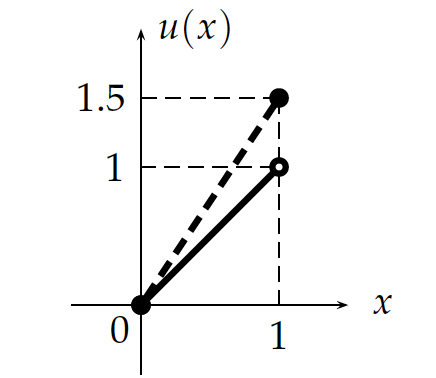
\includegraphics[scale = 0.4]{Images/sol.png}
    \label{fig:3}
  \end{figure}
  \noindent
  This problem has no solution, because the slope of $u(x)$ is 1 and
  at the boundary we have $u(1) = 1.5$. This means, we cannot find a
  solution that satisfies this Dirichlet Problem. This can be seen
  from the compatibility condition defined by
  (\ref{eq:13})-(\ref{eq:14}), as
  \begin{eqnarray}
    \lvert \varphi(1) - \varphi(0) \rvert = 1.5 \ge L(0,1) =
    \int_{0}^{1} 1 ds = 1
  \end{eqnarray}
  which does not satisfy the Compatibility condition (\ref{eq:14}).
\end{example}

\section{Comparison Theorem}
In this last section of the chapter, we study the uniqueness of the
solution to the Hamilton Jacobi Equation. We start with the classical
comparison principle to illustrate how uniqueness can be proved for
classical solutions. We then try to extend it to the viscosity setting
to study the uniqueness of the viscosity solution. Ishii\cite{ishii} in his work
presented and proved a comparison principle. Refer\cite{yong} for a detailed
version for the proof of the comparison theorem.

\subsection{Classical Comparison Theorem}
The classical version of the comparison theorem, involves assuming two
distinct solutions $u_1$ and $u_2$ solving the PDE, eventually showing
that they are equal. This is done by showing that,
\begin{equation}
  u_1 \le u_2, \quad u_2 \le u_1 \qquad in \;\;\; \bar{\Omega}
\end{equation}

\noindent
Refer \cite{yong} to see how this is done. The procedure followed here does not work for proving uniqueness for non-differentiable
solutions like $u(x) = \lvert x \rvert$, as the classical derivatives
are no longer defined at points of non-differentiability. To define
this in the viscosity setting, we have our new comparison theorem, by Ishii\cite{ishii}.

\subsection{Comparison Theorem}
In this section we state the formal statement of the comparison
theorem and see how that is used to conclude the uniqueness of the
viscosity solution.\\

\noindent
Before we state the theorem, we give the definition of modulus and a
couple of Hypothesis on the Hamiltonian $H$. Consider the following
HJE, with an Eikonal type Hamiltonian.
\begin{equation}
  H(x,Du(x)) = 0
\end{equation}

\begin{definition}
  \textbf{Modulus}: A function $m:[0,\infty[ \to [0,\infty[$ is called
  a modulus if its continuous and non-decreasing and satisfies $m(0) =
  0$
\end{definition}

\noindent
The two Hypothesis (H1) and (H2) on the Hamiltonian are stated below.
\begin{enumerate}
\item
  (H1) There is a modulus $m$ such that
  \begin{equation}
    \lvert H(x,p) - H(y,p)\rvert \le m (\lvert x-y \rvert (1+\lvert p \rvert))
  \end{equation}
  for $x,y \in \Omega$ and $p \in \mathbb{R}^n$
\item
  (H2) The function $p \to H(x,p)$ is convex on $\mathbb{R}^n$ for
  each $x \in \Omega$.

\end{enumerate}

\begin{theorem}
  \textbf{Comparison Theorem}\\

  \noindent
  Let $\Omega$ be a bounded open subset of $\mathbb{R}^n$. Assume that
  (H1) and (H2) holds. Let $\bar{u}$ and $\underset{\bar{}}{u} \in
  C^0$, respectively be viscosity super- and sub- solutions with
  \begin{equation}
    \underset{\bar{}}{u} \le \bar{u} \quad \text{on} \;\; \partial \Omega
  \end{equation}

  \noindent
  Also assume that\\

  (H3) $\exists$ a function $\varphi \in C^1(\Omega) \cap
  C^0(\bar{\Omega})$ such that, $\varphi \le \underset{\bar{}}{u}$ in
  $\bar{\Omega}$ and
  \begin{equation}
    \sup_{x\in \omega} H(x,D\varphi(x)) < 0 \qquad \forall \omega
    \subset \subset \Omega
  \end{equation}

  \noindent
  then $\underset{\bar{}}{u} \le \bar{u}$ in $\Omega$
\end{theorem}

\noindent
With this, we have the uniqueness result,
\begin{theorem}
  Let $u,v$ be two viscosity solutions of the Eikonal type HJE, such
  that $u = v \;\;\text{on} \;\;\partial \Omega$. Then $u = v$. Thus,
  the BVP,
  \begin{eqnarray}
    H(x,Du(x)) &=& 0 \qquad \text{in} \;\; \Omega\\
    u(x) &=& \varphi(x) \qquad \text{on} \;\; \partial \Omega
  \end{eqnarray}
  has atmost one viscosity solution.\\

  \noindent
  \textbf{Proof:} The proof is a direct consequence of the comparison
  theorem. As $u$ and $v$ are both viscosity sub- and super-solutions,
  by the comparison principle, $u \le v$ and $v \le u$ on $\Omega$. This implies
  $v = u$ on $\Omega$.
\end{theorem}


	\chapter{Orthographic Shape from Shading}
	% chapters/osfs.tex
%  Third chapter in osfs.tex

\section{Mathematical formulation of the Model}
One of the first attempts to solve this classical inverse problem was by Berthold K.P Horn by finding solutions of nonlinear first order partial differential equation called the \emph{brightness equation} under specific assumptions. This \emph{brightness equation} in simple words can be described as the map between the image intensities to the slope of the unknown surface, so that the shape can be constructed from the shading.\\

\noindent From Figure (\ref{fig:5}), in an orthographic camera model the surface point is directly projected onto the retinal plane in contrast to the perspective model which will be discussed in detail in Chapter $4$.\\

  \begin{figure}[h!]
  	\centering
  	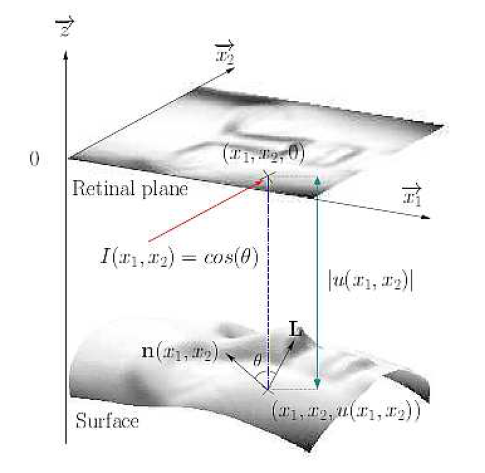
\includegraphics[scale = 0.3]{Images/orthographic_model.png}
  	\caption{Orthographic camera model}
  	\label{fig:5}
  \end{figure}
\pagebreak

\noindent The modelling of the problem leads to a partial differential equation. This equation arises from the following
\begin{equation}
I(x_1,x_2) = R(n(x_1,x_2))
\end{equation}	
where $(x_1,x_2)$ are the coordinates of a point $x$ in the image. The brighness equation is the relation between the reflectance map ($R$) to the brightness intensity ($I$). Almost all the shape from shading methods assume that the surface is \emph{Lambertian}. In this case, the reflectance map is the cosine of the angle between the light vector $\textbf{L}(x)$ and the normal vector $\textbf{n}(x)$ to the surface.
\begin{equation}
R = \cos(\textbf{L,n}) = \frac{\textbf{L}}{\lvert\textbf{L}\rvert}\cdot \frac{\textbf{n}}{\lvert\textbf{n}\rvert}
\end{equation}

\noindent Let $\Omega$ be an open subset of $ \mathbb{R}^2$ representing the image domain. For example $]a,b[ \times ]c,d[$.
\noindent In the Orthographic model we assume the light vector to be constant. We assume the light source to be unique and punctual. For $y \in \mathbb{R}^3$ , we denote $\mathbf{L}(y)$ the unit vector representing the light source direction at the point $y$. If the light source is located at infinity then the light vector field is uniform (i.e. constant). In this case, we denote by $\textbf{L} = (\alpha, \beta, \gamma)$ with $\gamma > 0$ and $\textbf{l} = (\alpha ,\beta)$. \\

\noindent Let us denote by $u$ the distance of the points in the scene to the camera. Now we have $\mathbf{n}(x) = (-\nabla u, 1)$. The SFS problem is then, given $I$ and \textbf{L}, to find a function $ u : \bar{\Omega} \rightarrow \mathbb{R}$ satisfying the brightness equation
\begin{equation}
	\forall x \in \Omega,  I(x) = \frac{-\nabla u(x) \cdot \mathbf{l} + \gamma}{\sqrt{1 + \lvert \nabla u(x) \rvert ^2}}
\end{equation}

\noindent This equation is rewritten, where $ p = \nabla u $. 
\begin{equation}
	H(x,p) = I(x)\sqrt{1+\lvert p \rvert^2} + p\cdot 1 - \gamma
\end{equation}
\noindent In our case we have considered a case where \textbf{L} = $(0,0,1)$ to obtain a Eikonal type equation where the function $H$ is called the \emph{Hamiltonian}.
\begin{equation}
	H_{Eiko} (x,p) = \lvert p \rvert - \sqrt{\frac{1}{I(x)^2} - 1}
\end{equation}

\section{Problem of Uniqueness}
\noindent Now consider the Eikonal equation in 1D,
\begin{eqnarray}
	\lvert u'(x)\rvert = 1 \qquad x\in (-1,1)\\
	u = 0 \qquad x\in \{-1,1 \}
\end{eqnarray}
\noindent The Hamiltonian $H(x,p) = \lvert p\rvert -1$ where $p=\nabla u$, is a covex function in $p$. We now show that the solution $u^+(x) = 1 - \lvert x\rvert$ is the viscosity solution to the problem.

\noindent \textbf{Proof:} Let $u-\phi$ attain maximum at $x_0$. In this case $x_0 = 0$.
\noindent This means,
\begin{eqnarray}
	u(x_0) - \phi(x_0) &\ge& u(x) - \phi(x) \qquad \forall x\in (-1,1) \\
	\implies \phi(x) - \phi(x_0) &\ge& u(x) - u(x_0)
\end{eqnarray}
\noindent If $x>x_0 =0$
\begin{eqnarray}
	\frac{\phi(x) - \phi(x_0)}{x-x_0} &\ge& \frac{u(x)-u(x_0)}{x-x_0} \\
	\implies \lim_{x\to x_0} \frac{\phi(x) - \phi(x_0)}{x-x_0}& \ge& \lim_{x\to x_0}\frac{u(x)-u(x_0)}{x-x_0}\\
	\phi' (x) &\ge& -1
\end{eqnarray}
\noindent If $x<x_0$, we follow the same procedure to get,
\begin{equation}
	\phi'(x) \le 1
\end{equation}
\noindent We get $\lvert \phi'(x)\rvert \le 1$, which shows that $u^+$ is a sub-solution to the Eikonal equation. One can verify that $u^+$ satisfies the super-solution condition as well and thus is a viscosity solution to the problem, which completes the proof.

\noindent It is easy to see that, by using the same steps, that $u^-(x) = \lvert x\rvert -1$ is \textbf{not a viscosity solution} if we choose the Hamiltonian $ H(x,p) = \lvert p\rvert -1$, but is indeed a viscosity solution for the Hamiltonian $H(x,p) = 1 - \lvert p \rvert$. Thus the viscosity solution is dependent on the nature of the Hamiltonian we choose, i.e., (concave or convex).

\noindent Let us consider the special case where the Eikonal equation is,
\begin{equation}
	\lvert \nabla u\rvert = 0
\end{equation}
\noindent This particular PDE presents us with a huge problem of \textbf{uniqueness}. This is evident from the sub-solution definition, that
\begin{eqnarray}
	H(x.\nabla\phi) \le 0 \\
	\implies \lvert \nabla\phi\rvert \le 0
\end{eqnarray}
\noindent which cannot be satisfied for all cases, as $\lvert\nabla\phi\rvert \ge 0$. This particular case is a problem when we consider the numerical solution of the Shape from Shading Model proposed by Rouy and Tourin \cite{rouy}.

\noindent Subsolution condition is satisfied as long as $0 < I(x) < 1$, and the uniqueness is lost as soon as $I(x) = 1$. These places where $I(x) = 1$ are called the \textbf{singularity points} where \emph{the solution has to specified in order to obtain the relevent solution}.

	\chapter{Perspective Shape from Shading}
	In this chapter, we deal with the perspective camera approach to Shape
from Shading problems. This approach differs from the Orthographic
Approach and can be considered to be a much more realistic approach to
shape from shading. In orthographic projection, we assume that the
light direction is given by a single vector $\mathbf{L} = (\alpha,
\beta, \gamma)$ and that the light rays are parallel to the retinal
plane. In perspective projection model, however the light rays are not
assumed to be parallel in case of perspective projection. This enables
us to reduce the number of singular points in the image. See Figure
(\ref{fig:2})
\begin{figure}[h!]
  \centering
  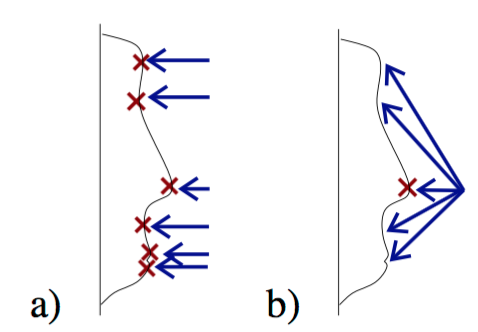
\includegraphics[scale = 0.5]{images/ovsp.png}
  \caption{a) Orthographic vs b) Perspective :
    Number of Singular Points}
  \label{fig:2}
\end{figure}

\noindent
In the perspective projection, the camera can be assumed to be placed at
the \textbf{focal point}, or at \textbf{infinity}. Prados and
Faugeras\cite{prados1} obtained a generic Hamiltonian for a perspective camera
approach  that unifies these conditions. However, the approach still
had the problem of singular points and the information at these points
must be specified apriori at these points to single out the unique
solution. So, Prados et.al\cite{prados2} came up with a modified brightness
equation to remove the notion of singular points. In this chapter, we
discuss the derivation of the HJE that describes the model, and
address existence and uniqueness of a viscosity solution.

\section{Mathematical Model}
In this section, we derive the Hamilton Jacobi Equation for
perspective model, using the modified brightness equation\cite{prados2}. Let
$\Omega \subset \mathbb{R}^2$. Let the scene be described by a
surface $\mathbb{S}$, which is parametrized by a function $S : \Omega
\to \mathbb{R}^3$,
\begin{equation}
  \mathbb{S} = \{S(x), \;\; x \in \bar{\Omega}\}
\end{equation}
Now, let us assume that the light source is placed on the focal
point. Figure (\ref{fig:3a}) represents the current setup in a
perspective projection model.\\
\begin{figure}
  \begin{subfigure}{0.5\textwidth}
    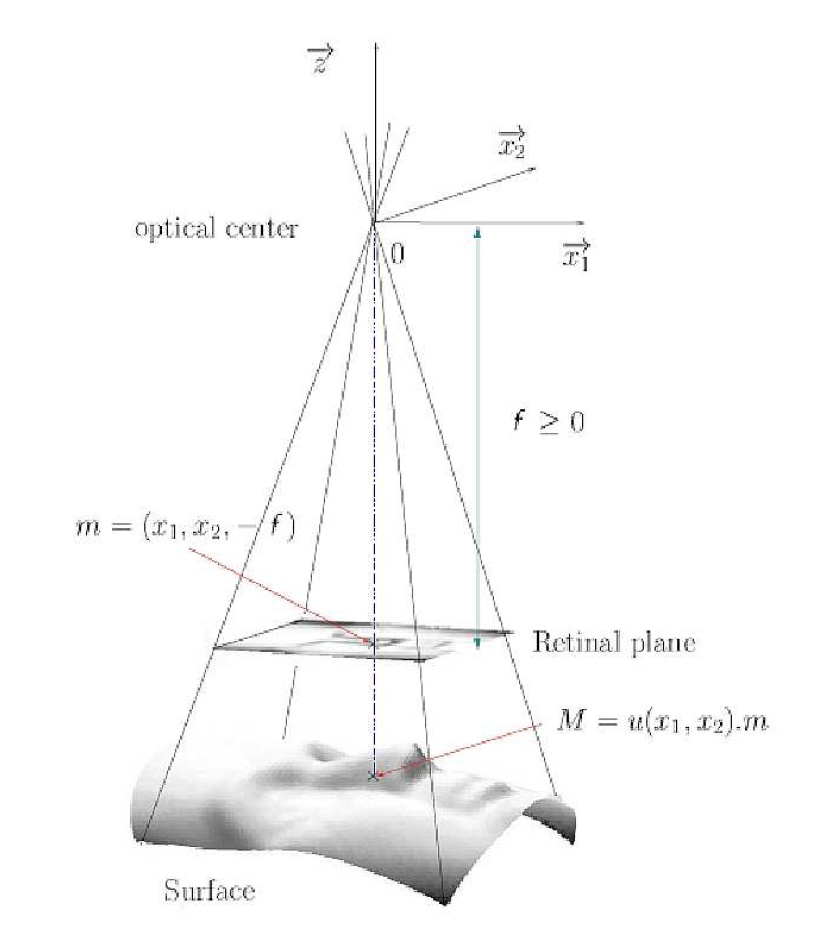
\includegraphics[scale = 0.5]{images/persp2.png}
    \subcaption{The scene}
    \label{fig:3a}
  \end{subfigure}
  \begin{subfigure}{0.5\textwidth}
    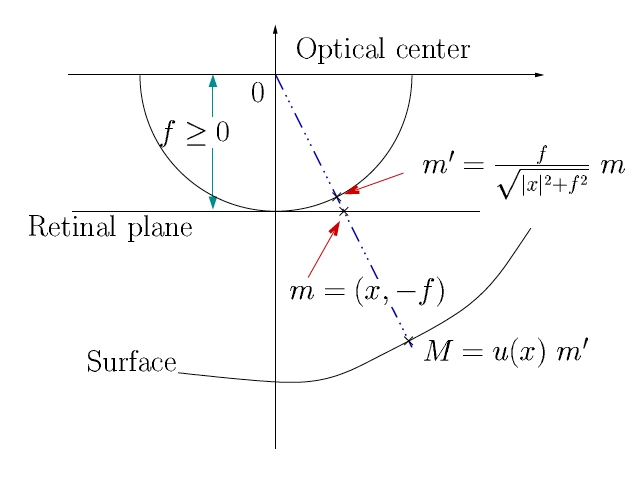
\includegraphics[scale = 0.65]{images/persp1.png}
    \subcaption{Surface representation}
    \label{fig:3b}
  \end{subfigure}
  \caption{Perspective Projection Model}
\end{figure}

\noindent
From Figure (\ref{fig:3b}), we can deduce that the parametrization of
the surface is given by,
\begin{equation}
  S(x) = \frac{fu(x)}{\sqrt{\lvert x \rvert^2 + f^2}} (x,-f)
\end{equation}

\noindent
where $f$ is the focal length of the camera. To simplify the model, Prados et.al in their previous work\cite{prados1}, used the
brightness equation
\begin{equation}
  R(x) = \cos \theta \label{eq:15}
\end{equation}
where $\theta$ is the angle between the Light Vector and the surface
unit normal and $R(x)$ is the irradiance of the surface. This gave a HJE which
suffered from singular points. So to overcome this difficulty, Prados
et.al\cite{prados2} did not neglect the $\frac{1}{r^2}$ attenuation term in their
model, which would normally be neglected to simplify the
model. Contrary to this statement, adding the attenuation term would
make the model better posed.\\

\noindent
The image irradinace equation (\ref{eq:15}), now becomes,
\begin{equation}
  R(x) = \frac{\cos \theta}{r^2}\label{eq:16}
\end{equation}
where $r = fu(x)$ is the distance between the light source and the considered
surface point $u(x)$. Assuming that the surface is lambertian and the camera is placed at the focal point, we have the unit light vector $L$ and the
surface unit normal $n$,
\begin{eqnarray}
  L(S(\mathbf{x})) &=& \frac{1}{\sqrt{\lvert \mathbf{x} \rvert^2+f^2}} (\mathbf{x},-f)\label{eq:17}\\
  n(\mathbf{x}) &=& \left( f\nabla u(\mathbf{x}) -
  \frac{fu(\mathbf{x})}{\lvert \mathbf{x} \rvert^2 + f^2} \mathbf{x},\;\;
  \nabla u(\mathbf{x}).\mathbf{x} + \frac{f u(\mathbf{x})}{\lvert
  \mathbf{x} \rvert^2 + f^2} f\right)\label{eq:18}
\end{eqnarray}

\noindent
Using (\ref{eq:16}) - (\ref{eq:18}), and $I(\mathbf{x}) = \cos \theta = L(\mathbf{x}).n(\mathbf{x})$, we
obtain the equation,
\begin{equation}
  I(\mathbf{x})f^2 \frac{\sqrt{f^2|\nabla u(\mathbf{x})|^2 + (\nabla
      u(\mathbf{x}).\mathbf{x})^2/Q(\mathbf{x})^2 +
      u(\mathbf{x})^2}}{u(\mathbf{x})} - u(\mathbf{x})^{-2} = 0
\end{equation}

\noindent
Assuming that the surface is visible, that is $u(\mathbf{x}) > 0$, we
make a change of variables $v = \ln u$. This gives us the HJE,
\begin{equation}
  -e^{-2v} + \frac{I(\mathbf{x})f^2}{Q(\mathbf{x})} \sqrt{f^2 |\nabla
    v(\mathbf{x})|^2 + (\nabla v(\mathbf{x}). \mathbf{x})^2 +
    Q(\mathbf{x})^2} = 0 \label{eq:19}
\end{equation}
where $Q(\mathbf{x}) = \sqrt{\frac{f^2}{|\mathbf{x}|^2 +
    f^2}}$. (\ref{eq:19}) is the HJE that describes the
setting. Solving for $u(\mathbf{x})$ with the known parameters $f,I$
gives the reconstructed 3D object. In the next section, we briefly
discuss the existence and uniqueness of the solution to (\ref{eq:19}).

\section{Existence and Uniqueness}
Consider the following Dirichlet boundary value problem,
\begin{eqnarray}
  -e^{-2v} + \frac{I(x)f^2}{Q(x)} \sqrt{f^2|\nabla u|^2 + (x.\nabla
    u)^2 + Q(x)^2} = 0 \qquad \text{in} \;\;\; \Omega \label{eq:20}\\
  u(x) = \varphi(x) \qquad \text{on} \;\;\; \partial \Omega \label{eq:21}
\end{eqnarray}

\noindent
Let us denote the Hamiltonian of the problem by $H(x,v,p)$, $p =
\nabla v$. The following two theorems gives the condition for the
existence and uniqueness of solution to the Prados model.
\begin{theorem}
  \textbf{Existence of continuous viscosity solution to the Prados
    Model}\\
  If
  \begin{itemize}
  \item
    (A1) \textbf{Regularity} : $H \in C^0(\bar{\Omega} \times \mathbb{R}^n)$
  \item
    (A2) \textbf{Convexity} : $H$ is convex with respect to $\mathbf{p} \;\;\forall
    \;\;\mathbf{x} \in \bar{\Omega}$
  \item
    (A3) \textbf{Subsolution} : $\inf_{\mathbf{p} \in \mathbb{R}^2}
    H(\mathbf{x},u,\mathbf{p}) \le 0 $ in $\bar{\Omega}$
  \item
    (A4) \textbf{Uniform Coercivity} : $H(\mathbf{x},u,\mathbf{p}) \to +\infty$
    when $|\mathbf{p}| \to \infty$ uniformly with respect to $x \in
    \bar{\Omega}$.
  \item
    (A5) $u(\mathbf{x}) = \varphi(\mathbf{x})$ satisfies the compatibity condition.
  \end{itemize}
  then $u$ is a continuous viscosity solution of the Hamilton Jacobi Equation.
\end{theorem}

\begin{theorem}
  \textbf{Uniqueness of solution to the Prados
    Model}\\
  If
  \begin{itemize}
  \item
    (A1) \textbf{Convexity} : $H$ is convex with respect to $\mathbf{p} \;\;\forall
    \;\;\mathbf{x} \in \bar{\Omega}$
  \item
    (A2) \textbf{Space variable regularity} : There exists a modulus $m$ such
    that $\forall \mathbf{x},\mathbf{y} \in \bar{\Omega}$ and
    $\mathbf{p}\in\mathbb{R}^2$, $|H(\mathbf{x},u,\mathbf{p}) -
    H(\mathbf{y},u,\mathbf{p})| \le m(|x-y|(1+|p|))$
  \item
    (A3) \textbf{Strict Subsolution} : There exists a strict viscosity
    subsolution $\underset{\bar{}}{u}$, such that
    $H(\mathbf{x},\underset{\bar{}}{u}, \mathbf{p}) < 0 \;\; \forall
    \;\; \mathbf{x}\in\Omega$
  \end{itemize}
  then there exists atmost one continuous viscosity solution to the
  HJE such that $u(\mathbf{x}) = \varphi(\mathbf{x})$ on the boundary.
\end{theorem}

\noindent
A rigorous proof for existence and uniquness can be found
in \cite{prados2}. Most of the conditions like convexity and regularity of the
Hamiltonian can be easily verified. The most interesting property in
the theorem is the subsolution condition. The Hamiltonian $H(x,u,p)$
satisfies the subsolution condition, if
\begin{eqnarray}
  &\implies&\inf_{p\in\mathbb{R}^2}H(x,u,p) \le 0 \\
  &\implies& -e^{-2u} + I(x)f^2 \le 0 \quad \forall \;\; x \in \Omega\\
  &\implies& I(x)f^2 \le e^{-2v} \\
  &\implies& v \le -\frac{1}{2} \ln (I(x)f^2) \label{eq:22}
\end{eqnarray}

\noindent
(\ref{eq:22}) can be reformulated as
\begin{equation}
  \implies v_0 = -\frac{1}{2}\ln(\min_{x\in\Omega} I(x)f^2) \label{eq:23}
\end{equation}

\noindent
(\ref{eq:22}) assures that a unique viscosity solution exists to the
problem. (\ref{eq:23}) can be supplied as an initial condition to evolution
type schemes to ensure convergence of the numerical scheme to the
exact solution. The notion of singular points disappear in this case as
long as (\ref{eq:22}) is satisfied. This is not assured in other cases\cite{prados1,prad,prad2}
because of the absence of the $e^{-2u}$ term in the Hamiltonian and
thus the subsolution condition is violated at these points. Thus, this
model has a unique viscosity solution that satisfies the HJE in
$\Omega$ and $\varphi(x)$ on $\partial \Omega$.\\

\noindent
In the next chapter, we discuss the numerical schemes used to solve
Hamilton Jacobi Equations.


	\chapter{Numerical Schemes}
	In this chapter, we discuss some interesting numerical methods to
solve the Hamilton Jacobi Equations. First we start off with a brief
introduction to Hyperbolic Conservation Laws. In the next section, we
discuss some of the numerical techniques to solve Hyperbolic
Conservation Laws. In section 3, we discuss the numerical schemes to
solve Eikonal Type HJE, with the idea of conservation laws. Next, we discuss the numerical schemes to solve the Perspective Projection Model developed by Prados and Faugeras\cite{prados2}.


\section{Hyperbolic Conservation Laws}
Scalar Hyperbolic Conservation Laws in 1D is represented as
\begin{equation}
	u_t + f(u)_x = 0 \label{eq:24}
\end{equation}
where $f:\mathbb{R} \to \mathbb{R}$ is a smooth function known as Flux. If $u$ is a smooth function ,(\ref{eq:24}) can be written in a non-conservative form,
\begin{equation}
	u_t + f'(u)u_x = 0\label{eq:25}
\end{equation}
(\ref{eq:25}) when augmented with initial conditions $u(x,0) = u_0(x)$, can be solved with the \textbf{method of characteristics}. This is possible only if $f$ is linear. If $f$ is nonlinear, we have non-smooth solutions even if $f$ and $u_0$ are smooth. On using method of characteristics, we observe that the characteristics intersect at some point say P. At P the solution $u$ takes multiple values. These points where uniqueness breakdown are known as ``shocks". Thus it becomes insufficient to define the solution with the classical theory. So we are in a point to define ``weak solutions" to the PDE. For more details, we refer the reader to \cite{leve}.
\begin{definition}
	\textbf{Weak solution}\\
	
	\noindent
	Let $v : \mathbb{R} \times [0,\infty) \to \mathbb{R} $, be a smooth function with compact support. A bounded measurable function $u$ is said to be a weak solution to (\ref{eq:24}) if
	\begin{equation}
		\int_{0}^{\infty} \int_{-\infty}^{\infty} \left(uv_t + f(u)v_x\right) dxdt + \int_{-\infty}^{\infty} u v|_{t=0}dx = 0 \label{eq:26}
	\end{equation}
\end{definition}

\noindent
This is obtained directly by multiplying (\ref{eq:24}) with $v$ and then integrating over $R \times [0,\infty)$. If $u$ is a smooth and satisfies (\ref{eq:26}), then $u$ satisfies (\ref{eq:24}). We can show that the shock propogates with a speed $s$ along the discontinuity where,
\begin{equation}
	s = \frac{[f(u)]}{[u]}
\end{equation} 
and $[f(u)] = f(u_r) - f(u_l)$ is the jump in $f(u)$ across the discontinuity, $[u] = u_r - u_l$ is the jump in $u$ across the discontinuity. This condition is known as the \emph{Rankine-Hugniot Condition}. This states that, no matter what values $u_l$ and $u_r$ might take, the RH Condition must always be satisfied at the shock.\\

\noindent
But for (\ref{eq:24}), we may have more than one solution satisfying the RH-Condition. But only one solution is the physically relevant solution. This is known as the Entropy Solution (Analogous to the viscosity solution defined in Chapter 2). An entropy solution satisfies what is known as the entropy condition, which is defined below.
\begin{definition}
	\textbf{Entropy condition for convex flux}\\
	
	\noindent
	A discontinuity propogating with a speed $s$ satisfying the RH condition, satisfies the entropy condition if 
	\begin{equation}
		f'(u_l) > s > f'(u_r)
	\end{equation}
	which is equivalent to $u_l > u_r$ if $f$ is convex.
\end{definition}
\begin{definition}
	\textbf{Kruzkov Entropy condition}\\
	
	\noindent
	A discontinuity propogating with a speed $s$ satisfying the RH condition, satisfies the entropy condition if 
	\begin{equation}
	\frac{f(v) - f(u_l)}{v-u_l} > s > \frac{f(v) - f(u_r)}{v - u_r}
	\end{equation}
	This will hold for any flux function $f$.
\end{definition}

\noindent
Next, we define the \emph{Riemann Problem}. This will be used to construct the numerical schemes, where local Riemann Problems are solved in a finite volume and then patched up to get the solution to our problem.\\

\noindent
A conservation law, together with a piecewise constant data having a single discontinuity is known as a Riemann Problem.
\begin{eqnarray}
	u_t + f(u)_x &=& 0 \\
	u(x,0) &=& \left\{ 
		\begin{array}{ll}
			u_l  & x < 0 \\
			u_r & x > 0
		\end{array} 
		\right.
\end{eqnarray}

\noindent
The solution to the Riemman problem for any flux $f$ is given by\cite{leve},
\begin{eqnarray}
	u(x,t) &=& \left\{ 
	\begin{array}{ll}
	u_l  & x < tf'(u_l) \\
	(f')^{-1}\left(\frac{x}{t}\right) & tf'(u_l) < s < tf'(u_r)\\
	u_r & x > tf'(u_r)
	\end{array} 
	\right.
\end{eqnarray}

\section{Numerical Schemes for Hyperbolic Conservation Laws}
In this section, we see how to develop Finite Difference approximations to Hyperbolic conservation laws. First let us consider the problem,
\begin{eqnarray}
	u_t + f(u)_x &=& 0 \qquad \text{in} \;\; \mathbb{R} \times (0,\infty)\label{eq:28}\\
	u(x,0) &=& u_0(x) \qquad x \in \mathbb{R}\label{eq:29}
\end{eqnarray}

\noindent
Now we discretize the $x$ axis by $\left\{x_{i+\frac{1}{2}}\right\}$, where
\begin{equation}
	x_{i+\frac{1}{2}} = \left(i + \frac{1}{2}\right) h, \quad i \in \mathbb{Z}, h > 0
\end{equation}
and $t$ by $\left\{t_n\right\}$, where
\begin{equation}
	t_n = n \Delta t \quad n = 0,1,2,\dots
\end{equation}
Let $\lambda = \Delta t / h$. Let $v_i^n$ denotes the approximate solution at the point $\left(x_{i+\frac{1}{2}}, t_n\right)$. Thus the initial data $\{v_i^0\}$ is given by
\begin{equation}
	v_i^0 = \frac{1}{h} \int_{x_{i-1/2}}^{x_{i+1/2}} u_0(x) dx
\end{equation}

\noindent
Now, we define the following terms,
\begin{definition}
	A finite difference scheme is said to be in the conservative form, if there exists a continuous function $F: \mathbb{R}^{2k} \to \mathbb{R}$ such that
	\begin{equation}
		v_i^{n+1} = H(v_{i-k}^n, \dots,v_{i+k}^n) = v_i^n - \lambda \left(F_{i+1/2}^n - F_{i-1/2}^n\right)\label{eq:27}
	\end{equation}
	where $F_{i+1/2} = F(v_{i-k+1}^n, \dots, v_{i+k}^n )$. The function $F$ is called the numerical flux.
\end{definition}
\begin{definition}
	A finite difference scheme is said to be consistent with the conservation law if 
	\begin{equation}
		F(v,\dots,v) = f(v) \quad \forall v \in \mathbb{R}
	\end{equation}
\end{definition}

\noindent
For the convergence of a scheme to the entropy solution, Lax-Wendroff theorem\cite{gowda} says that the scheme must be in the conservative form and consistent. This ensures that the approximate solution $v_i^n$ converges to the entropy solution. For the proof of the theorem, we refer the reader to \cite{gowda}.

\subsection{The Godunov Scheme}
The Godunov Scheme for the numerical solution conservation law defined in (\ref{eq:28}) - (\ref{eq:29}) is given by \cite{gowda,leve},
\begin{eqnarray}
	v_j^{n+1} &=& v_j^{n} - \lambda \left(F^n_{j+1/2} - F^n_{j-1/2}\right)\label{conlaw}\\
	\text{where} \qquad F^n_{j+1/2} &=& f(w_R(0,v_j^n,v_j^{n+1}))
\end{eqnarray}
where $w_R$ is the solution to the Riemann Problem.\\

\noindent
For a convex flux $f$, the Godunov Flux is given by,
\begin{equation}
	F^G(u,v) = \max(f(\max(u,\theta)), f(\min(v,\theta))) \label{godunov}
\end{equation}
and for a concave flux $f$,
\begin{equation}
	F^G(u,v) = \min(f(\min(u,\theta)), f(\max(v,\theta)))
\end{equation}

\noindent
where $\theta = \min_{u \in \mathbb{R}} f(u)$. This scheme is stable under the CFL - Condition\cite{leve}
\begin{equation}
	\lambda \sup_{j} v_j \le 1 \label{cfl}
\end{equation}

\noindent
For the detailed derivation of the Godunov Scheme, one can refer \cite{leve}. We can show that the Godunov scheme is in the conservative form, is consistent, stable under the CFL condition and hence converges to the entropy solution and is a upwind scheme.\cite{leve}

\subsection{Lax-Friedrich Scheme}
For the conservative form of the scheme in (\ref{conlaw}), the \textbf{Lax Friedrich} Flux is given by
\begin{equation}
	F^{LF} (u,v) = \frac{1}{2} \left(f(u) + f(v) - \frac{1}{\lambda} (v - u)\right) \label{laxf}
\end{equation}

\noindent 
The Lax-Friedrich Scheme is consistent and stable under the CFL Condition (\ref{cfl}). Thus this scheme converges to the entropy solution. But Lax-Friedrich Scheme is not an upwind scheme.

\section{Godunov Scheme for the Eikonal Equation}
In this section, we see how the Eikonal Equation in 1D can be viewed as a conservation law, thus enabling us to use the schemes defined in the previous section.\\

\noindent
The Eikonal Equation in 1D is given by, 
\begin{eqnarray}
	\lvert u_x \rvert = 1
\end{eqnarray}

\noindent
To solve this equation, we add a transient term $u_t$ and solve it till the steady state is reached.
\begin{equation}
	u_t + \lvert u_x \rvert = 1 \label{eiko}
\end{equation}

\noindent
where $u = u(x,t)$. Now set $v = u_x$. Differentiating (\ref{eiko}) paritally with respect to $x$, we get
\begin{eqnarray}
	&(u_t)_x& + \;\;(\lvert u_x \rvert)_x = 0\nonumber\\
	\implies &(u_x)_t& + \;\;(\vert u_x \rvert)_x = 0\nonumber\\
	\implies & v_t& + \;\;(\lvert v \rvert)_x = 0 \label{conlaw2}
\end{eqnarray}

\noindent
(\ref{conlaw2}) is precisely the conservation law, with $f(u) = \lvert u \rvert$. On using the Godunov scheme defined by (\ref{conlaw}), we have
\begin{equation}
	u_i^{n+1} = u_i^{n}	 - \Delta t \;\left(F^G\left(0,\frac{u_{i}^n - u_{i-1}^n}{h},\frac{u_{i+1}^n - u_{i}^n}{h}\right) -1 \right)
\end{equation}

\noindent
As $f(u) = \lvert u \rvert$ is a convex function, we can say that
\begin{equation}
	F^G(u,v) = \max(f(\max(u,0)), f(\min(v,0)))
\end{equation}

\noindent
This idea can be extended to the 2D case as well. For the Eikonal Equation
\begin{eqnarray}
	u_t + \sqrt{\left(\frac{\partial u }{\partial x}\right)^2 + \left(\frac{\partial u }{\partial y}\right)^2}  = 1
\end{eqnarray}
we can use the Godunov Flux to approximate the derivatives along each direction. So the scheme would become
\begin{eqnarray}
	u_{i,j}^{n+1} = u_{i,j}^n - \Delta t \; \left(\sqrt{F^{G_x}(0,D^-x,D^+x)^2 + F^{G_y}(0,D^-y,D^+y)^2} - 1\right)
\end{eqnarray}
where $D^\pm x$ and $D^\pm y$ denotes the forward and backward differences along $x$ and $y$ respectively. This scheme is consistent, stable under the CFL condition $\Delta t \le \min(h_x,h_y)$. \\

\noindent
This can be extended to the Hamiltonian defined by Prados in \cite{prados2} as well. The derivatives have to be replaced by the appropriate Fluxes to get the explicit scheme. The second term can be upwinded ($D^x$ and $D^y$) according to the derivative formula chosen by the Godunov Flux. One can easily verify that the scheme to solve the model is given by,
	\begin{equation}
		v_{i,j}^{n+1} = v_{i,j}^n - \Delta t \left(-e^{-2v_{i,j}} + J(x_i,y_j) \sqrt{f^2\left( \left(F^{G_x}\right)^2 + \left(F^{G_y}\right)^2\right)  + \left(x_iD^x + y_jD^y\right)^2 + Q(x_i,y_j)^2} \right) \label{eq:upw}
	\end{equation}\\

\noindent
The upwinding can be taken one-step further by taking $J(x,y)$ inside the square-root and upwinding $J(x,y)$ along with the derivatives. The results seem to be better when upwinding is done with $J(x,y)$ included inside the square root (Shown in Chapter 6) compared with the standard upwinding. In view of brevity, we just illustrate how the Godunov flux is modified.
\begin{equation}
	J_{i,j} \;F^{G_x}(0,D^+x,D^-x) \implies  F^{G_x}(0,J_{i+1,j}D^+x,J_{i,j}D^-x) \label{eq:upw1}
\end{equation}
where $J_{i,j} = J(x(i),y(j))$. Similarly upwinding is done in the $y$ direction. The second and the third term is multiplied by $J_{i,j}$ alone. 

	\chapter{Numerical Experiments}
	In this chapter we present some of the numerical results which we have obtained by using the convergent schemes discussed in the previous chapter. We give the results of the following,
\begin{itemize}
	\item
	1D Eikonal Equation
	\item
	Eikonal Equation in 2D.
	\item
	Solving Eikonal Equation on non-rectangular domains using the Immersed Boundary method.
	\item
	Results of the orthographic projection model.
	\item
	Results of the perspective projection model by Prados.	
\end{itemize}

\section{1D Eikonal Equation}
In this section, we present the solution to the most basic Hamilton Jacobi Equation. We use the Godunov Scheme defined in the previous chapter. This scheme converges to the unique viscosity solution, as it is consistent, stable, monotone and the original problem accepts a comparison principle \cite{yong}. Figure (\ref{fig:6}) shows the unique viscosity solution $u(x) = 1-\lvert x \rvert$ to the following Dirichlet Problem.
\begin{eqnarray}
	\lvert u' \rvert &=& 1 \qquad \text{in} \;\; (-1,1)\label{eq:30}\\
	u &=& 0 \qquad \text{on} \;\; \{-1,1\}\label{eq:31}
\end{eqnarray}
\begin{figure}
	\centering
	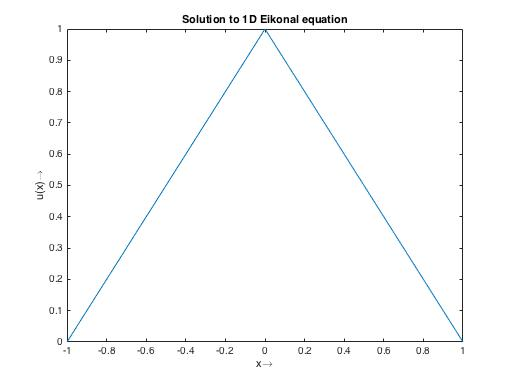
\includegraphics[scale=0.5]{Images/1deik/21.jpg}
	\caption{Viscosity Soution of the 1D Eikonal Equation}
	\label{fig:6}
\end{figure}

\noindent
The next figure (Figure (\ref{fig:7})) shows evolution of the solution to (\ref{eq:30}) - (\ref{eq:31}).\\
\begin{figure}[h!]
	\begin{subfigure}{0.5\textwidth}
		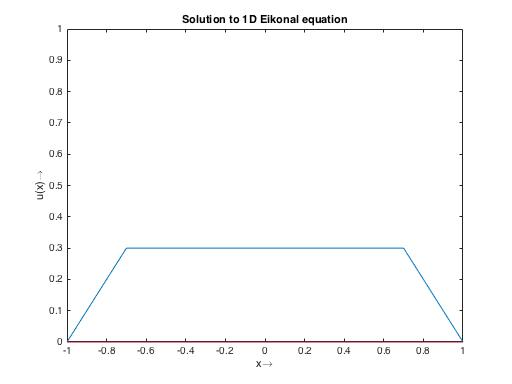
\includegraphics[scale = 0.4]{Images/1deik/3.jpg}
		\subcaption{n = 3 Iterations}
	\end{subfigure}
	\begin{subfigure}{0.5\textwidth}
			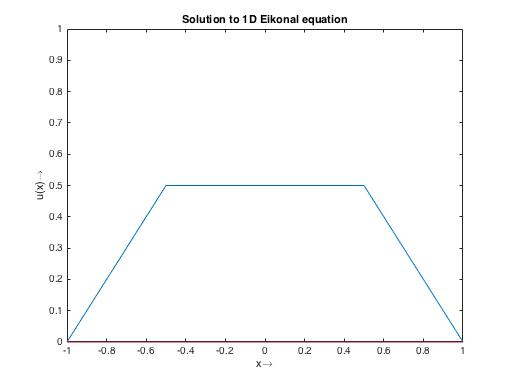
\includegraphics[scale = 0.4]{Images/1deik/5.jpg}
			\subcaption{n = 5 Iterations}
	\end{subfigure}
	\begin{subfigure}{0.5\textwidth}
			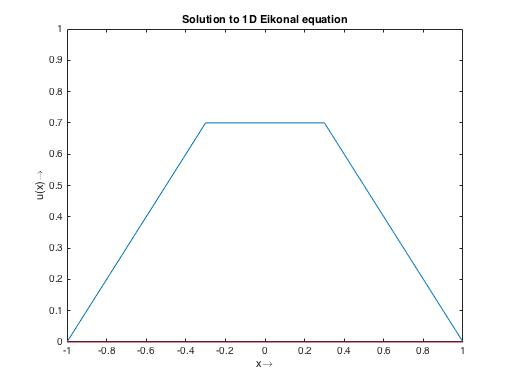
\includegraphics[scale = 0.4]{Images/1deik/7.jpg}
			\subcaption{n = 7 Iterations}
	\end{subfigure}
	\begin{subfigure}{0.5\textwidth}
			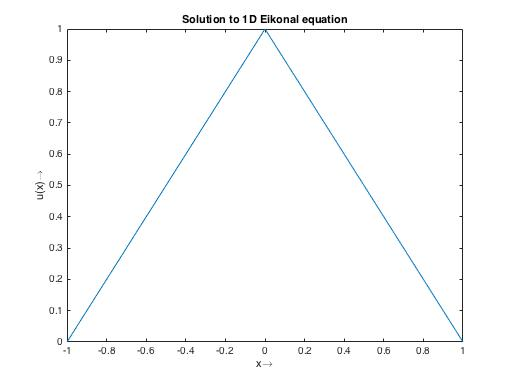
\includegraphics[scale = 0.4]{Images/1deik/21.jpg}
			\subcaption{n = 21 Iterations (Steady State $\epsilon = 10^{-16}$)}
	\end{subfigure}
	\caption{Evolution of solution to the Eikonal Equation. The steady state condition is taken as $\lVert U^{n+1} - u^{n} \rVert < \epsilon = 10^{-16}$}
	\label{fig:7}
\end{figure}

\pagebreak
\section{2D Eikonal Equation}
Next, we show the solution to the Eikonal Equation in 2D for a rectangular domain. For this, we have used the Godunov scheme as well, the fluxes approximating the derivatives along each directions.
\begin{eqnarray}
	\lvert \nabla u \rvert &=& 1 \qquad \text{in} \;\; \Omega = (-1,1) \times (-1,1)\\
	u &=& 0 \qquad \text{on}\;\;\partial \Omega
\end{eqnarray}

\noindent
Figure (\ref{fig:8}) shows the solution to the above Dirichlet Boundary Value Problem. We have taken a $50 \times 50$ mesh to solve the above problem.
\begin{figure}[h!]
	\centering
	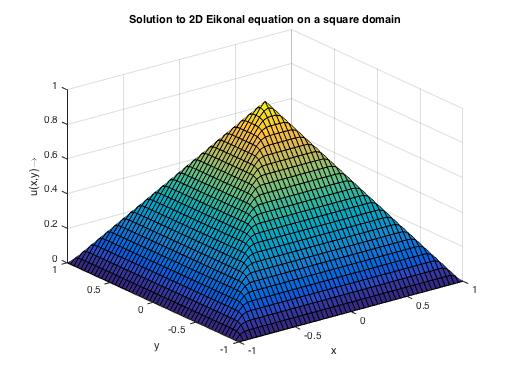
\includegraphics[scale = 0.5]{Images/2D_eik_square.jpg}
	\caption{Solution of 2D Eikonal Equation}
	\label{fig:8}
\end{figure}

\section{Immersed Boundary Method for 2D Eikonal Equations}
So far, the fintie difference techniques can be easily applied to a rectangular cartesian grid. The objective is to extend the same finite difference techniques to a variety other domains, for example - \textit{Circle, L-Domain, Circle with hole} etc. \\

\noindent
To illustrate the technique, we consider a circular domain. For comfort, let us consider a unit circle. We take a rectangular cartesian grid shown in Figure \ref{fig:1} and \textbf{``immerse"} the circluar domain into the rectangular mesh as shown in Figure \ref{fig:2}. This technique is known as the immersed boundary method \cite{pesk} which is widely used to solve problems in Fluid Mechanics.\\

\begin{figure}[h!]
	\centering
	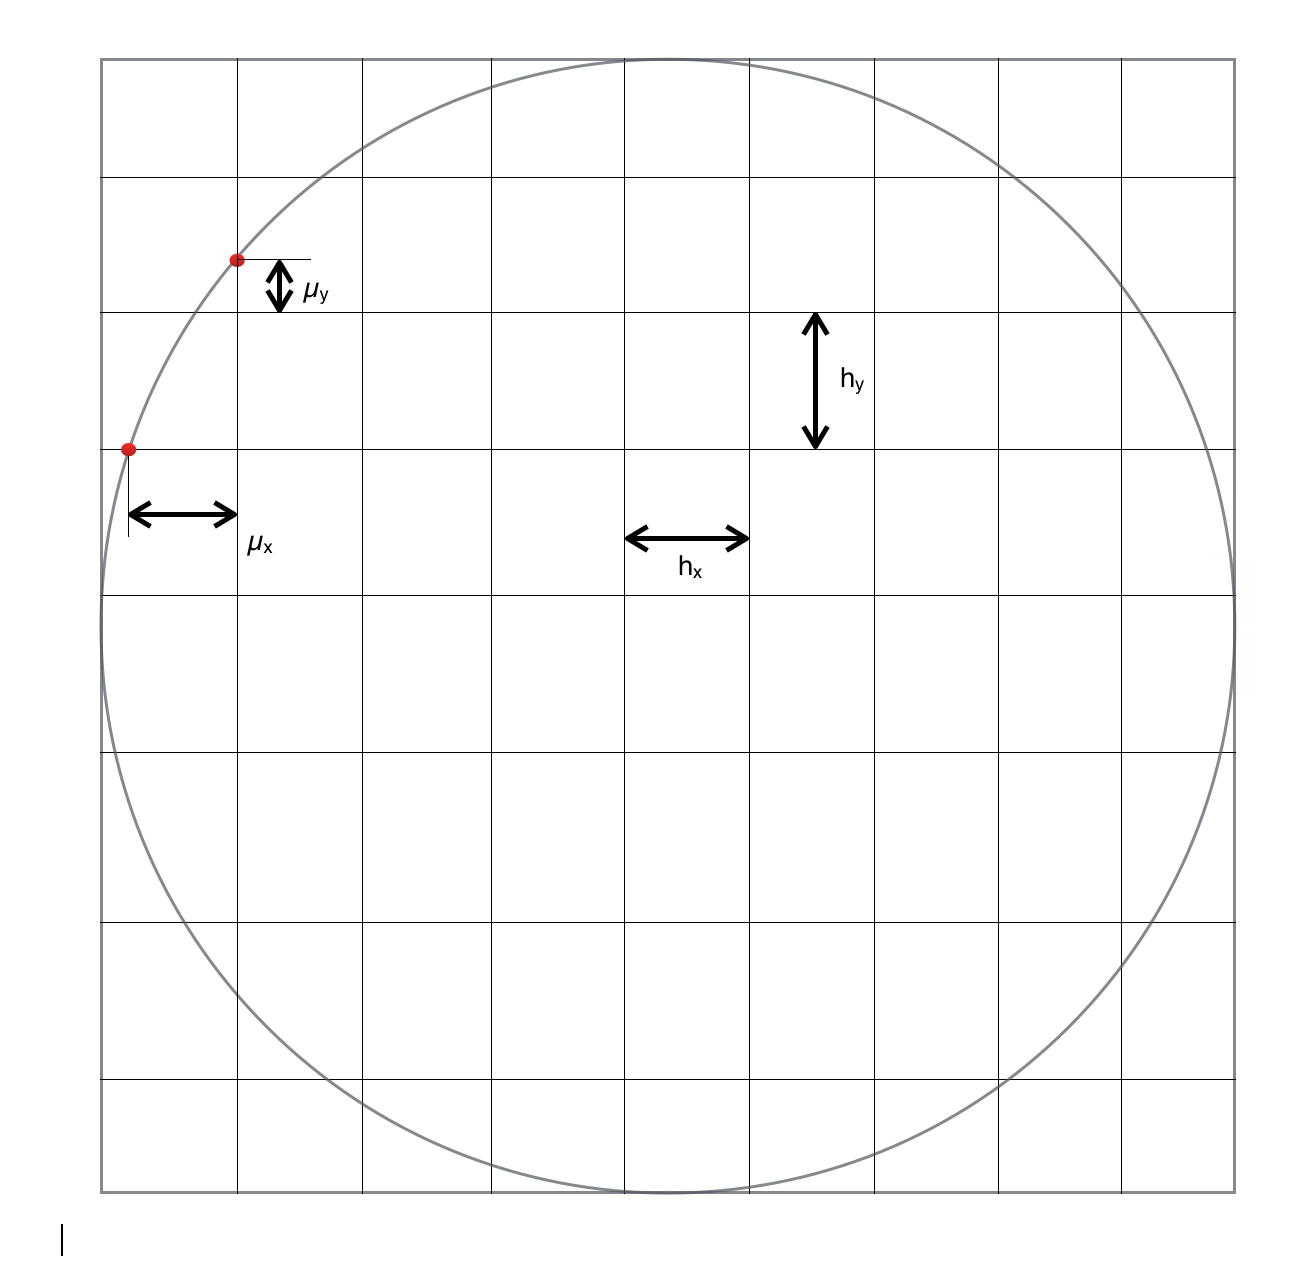
\includegraphics[scale=0.5]{Images/circle-immerse.png}
	\caption{Immersed Circle}
	\label{fig:9}
	\end{figure}
	
	\noindent
	The first challenge in this method is to track the interior and boundary of the 
	immersed domain. For this we introduce a data structure called the \textbf{inout} matrix. The \textbf{inout} matrix is defined as follows,
	\begin{equation}
	inout_{ij} = 
	\begin{Bmatrix}
	0, &\;\; \text{if} \;\; (x_i,y_j) \;\; \text{lies inside the immersed domain}\\
	1, &\;\; \text{otherwise}
	\end{Bmatrix}
	\end{equation}.
	
	\noindent
	The way to track the boundary of the immersed domain using the \textbf{inout} matrix is natural. We simply ignore the grid points whose \textbf{inout} entry is $1$ and set the value $u(x,y) = 0$ at those places. We then solve the eikonal equation using only inside the immersed boundary where the \textbf{inout} value is $0$.\\
	
	\noindent
	To apply the boundary conditions, we are in a position to obtain the points marked in \textbf{red} in Figure \ref{fig:9}. These points are easily obtained by solving the grid lines $x = -1 + ih_x$ or $y = -1 + jh_y$ with the equation of the circle. Note that, from the Dirichlet boundary condition, the value of $u(x,y)$ is prescribed in the problem at these points. \\
	
	\noindent
	When we apply the finite difference formula on the point which is immediately next to the \textbf{red} point - inside the domain, we are in a position to use the distances $\mu_x$ and $\mu_y$ to calculate the finite differences. This is the place where we choose to ignore the points outside the immersed boundary, and take the points that lie on the circle instead.\\
	
	\noindent
	With the distances $\mu_x$ and $\mu_y$, the update formula near the immersed boundary becomes,
	\begin{eqnarray}
	v_{ij}^{n+1} &=& v_{ij}^n - \Delta t\left(\sqrt{D_x^2 + D_y^2}-1\right)\\ 
	D_x &=& max\left(\frac{v_{i+1,j}-v_{i,j}}{\mu_1},\frac{v_{i-1,j}-v_{i,j}}{\mu_2},0\right)\\
	D_y &=& max\left(\frac{v_{i,j+1}-v_{i,j}}{\mu_3},\frac{v_{i,j-1}-v_{i,j}}{\mu_4},0\right)
	\end{eqnarray}
	where $\mu_{1,\dots,4}$ is chosen accordingly, depending on the position of top, bottom, left or right neighboring grid points. If the grid point above the current point, lies on the boundary, then $\mu_3 = \mu_y$ and $\mu_1 =  \mu_2 = h_x, \;\; \mu_4 = h_y$ and so on. There may be cases where two of the neighboring grid points may lie on the boundary. All those cases must be taken proper care of. Results of some numerical experiments are shown in the next chapter.
	
	\subsection{Results}
	Some Numerical Experiments were carried out using the Godunov scheme for a variety of domains.\\
			
		\noindent
		Numerical Experiments were conducted using \textbf{Fortran90} to find out the order of convergence of the scheme with $\epsilon = 10^{-16} \approx$ Machine Error. The \textbf{inout} matrix for a circle with a $10 \times 10$ mesh is shown in Figure \ref{fig:11}
		\begin{figure}[h!]
			\centering
			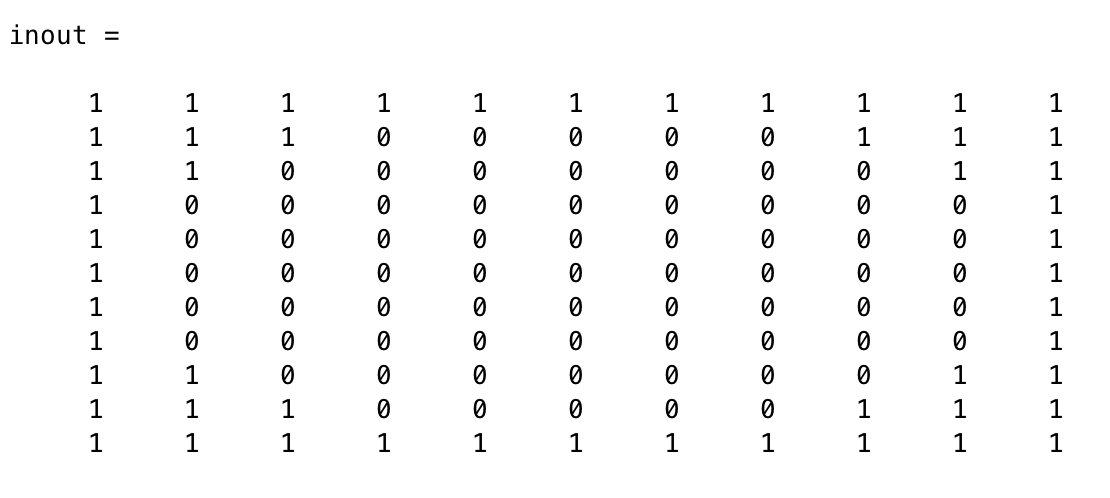
\includegraphics[scale=0.5]{Images/inout.png}
			\caption{\textbf{Inout} Matrix for $10 \times 10$ mesh}
			\label{fig:11}
			\end{figure}\\
			\noindent
			With this \textbf{inout} matrix, we compute the necessary distances near the boundary, for use in the Finite Difference Formula. Following is the profile, obtained when the Godunov Scheme is run for $50 \times 50$ mesh on the master rectangle with steady state $\epsilon = 10^{-16}$.
			\begin{figure}[h!]
				\centering
				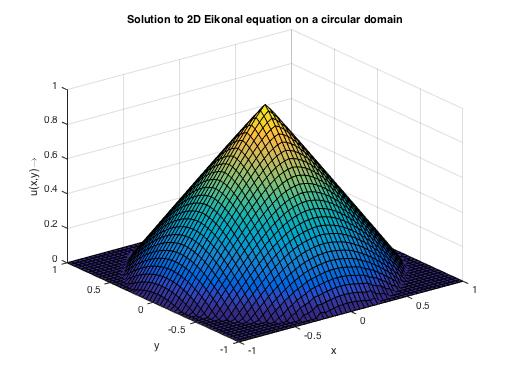
\includegraphics[scale = 0.5]{Images/2D_eik_circle.jpg}
				\caption{Solution in a circular domain}
				\label{fig:5}
				\end{figure}\\
				
				\noindent
				Using \textbf{Fortran90}, order of convergence analysis was performed on the scheme and the results are tabulated.\\
				\begin{center}
					\begin{tabular}{|c|c|c|}
						\hline
						N & Error & Order of Convergence\\
						\hline
						10 & 0.9878E-01 & 0.685 \\
						\hline
						20 & 0.6145E-01 & 0.728 \\
						\hline	
						40 & 0.3710E-01 & 0.738 \\
						\hline	
						80 & 0.2223E-01 & 0.761 \\
						\hline	
						160 & 0.1311E-01 & 0.783 \\
						\hline	
						320 & 0.0762E-01 & 0.800  \\
						\hline
						640 & 0.0437E-01 & -\\
						\hline
						\end{tabular}
						\end{center}
						
						\noindent
						The same method can be used to generate profiles for a variety of domains as shown. The idea is to tweak the \textbf{inout} matrix corresponding to the shape of the domain and appropriately take care of the immersed boundary grid points.\\
						
						\begin{figure}[h!]
							\begin{subfigure}{.5\textwidth}
								\centering
								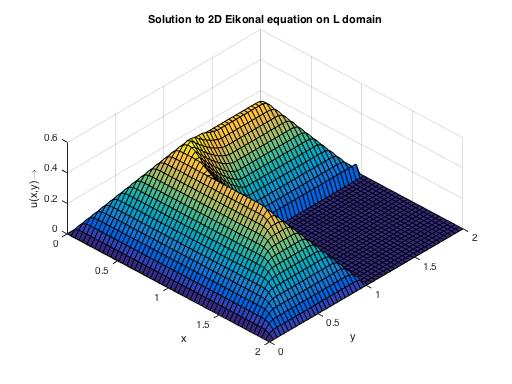
\includegraphics[scale = 0.45]{Images/2D_eik_Ldomain.jpg}
								\caption{L-Domain}
								\label{fig:12}
								\end{subfigure}
								\begin{subfigure}{.5\textwidth}
									\centering
									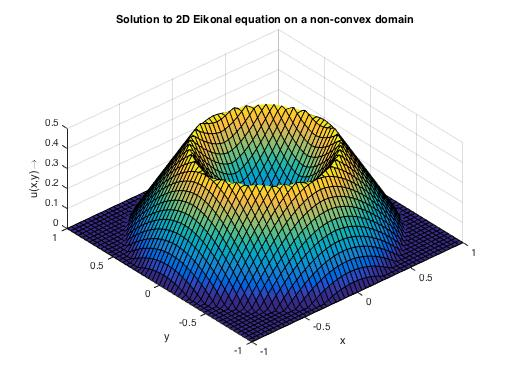
\includegraphics[scale = 0.45]{Images/2D_eik_hole.jpg}
									\caption{Circle with a hole in the middle}
									\label{fig:13}
									\end{subfigure}
									\caption{Other Domains}
									\end{figure}
									
									\noindent
									Figure \ref{fig:12} and Figure \ref{fig:13} shows the profile that is obtained when the Immersed Boundary Technique is applied to solve the Eikonal Equation on a L-Shaped Domain and a circle with a hole in it (non-convex domains) respectively. Similar Experiments can be conducted to model various problems in a variety of domains.

\section{Orthographic Projection}
For the orthographic projection model \cite{rouy}, the Eikonal Type HJE, is given by 
\begin{eqnarray}
	\lvert \nabla u \rvert = \sqrt{\frac{1}{I(x)^2} - 1}\label{eq:ortho}
\end{eqnarray}
where $I(x)$ is the intensity function of the input image. Following test was carried out to verify the model using a synthetic image of a vase shown in Figure (\ref{fig:14}). 
\begin{figure}[h!]
	\centering
	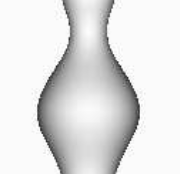
\includegraphics[scale = 1.5]{Images/vase.png}
	\caption{Synthetic Test Vase}
	\label{fig:14}
\end{figure}

\noindent
(\ref{eq:ortho}) was solved with a Homogeneous Neumann Boundary Condition on $\partial \Omega$ and the result is presented below. The equation was solved using the Godunov upwind scheme.
\begin{figure}[h!]
	\centering
	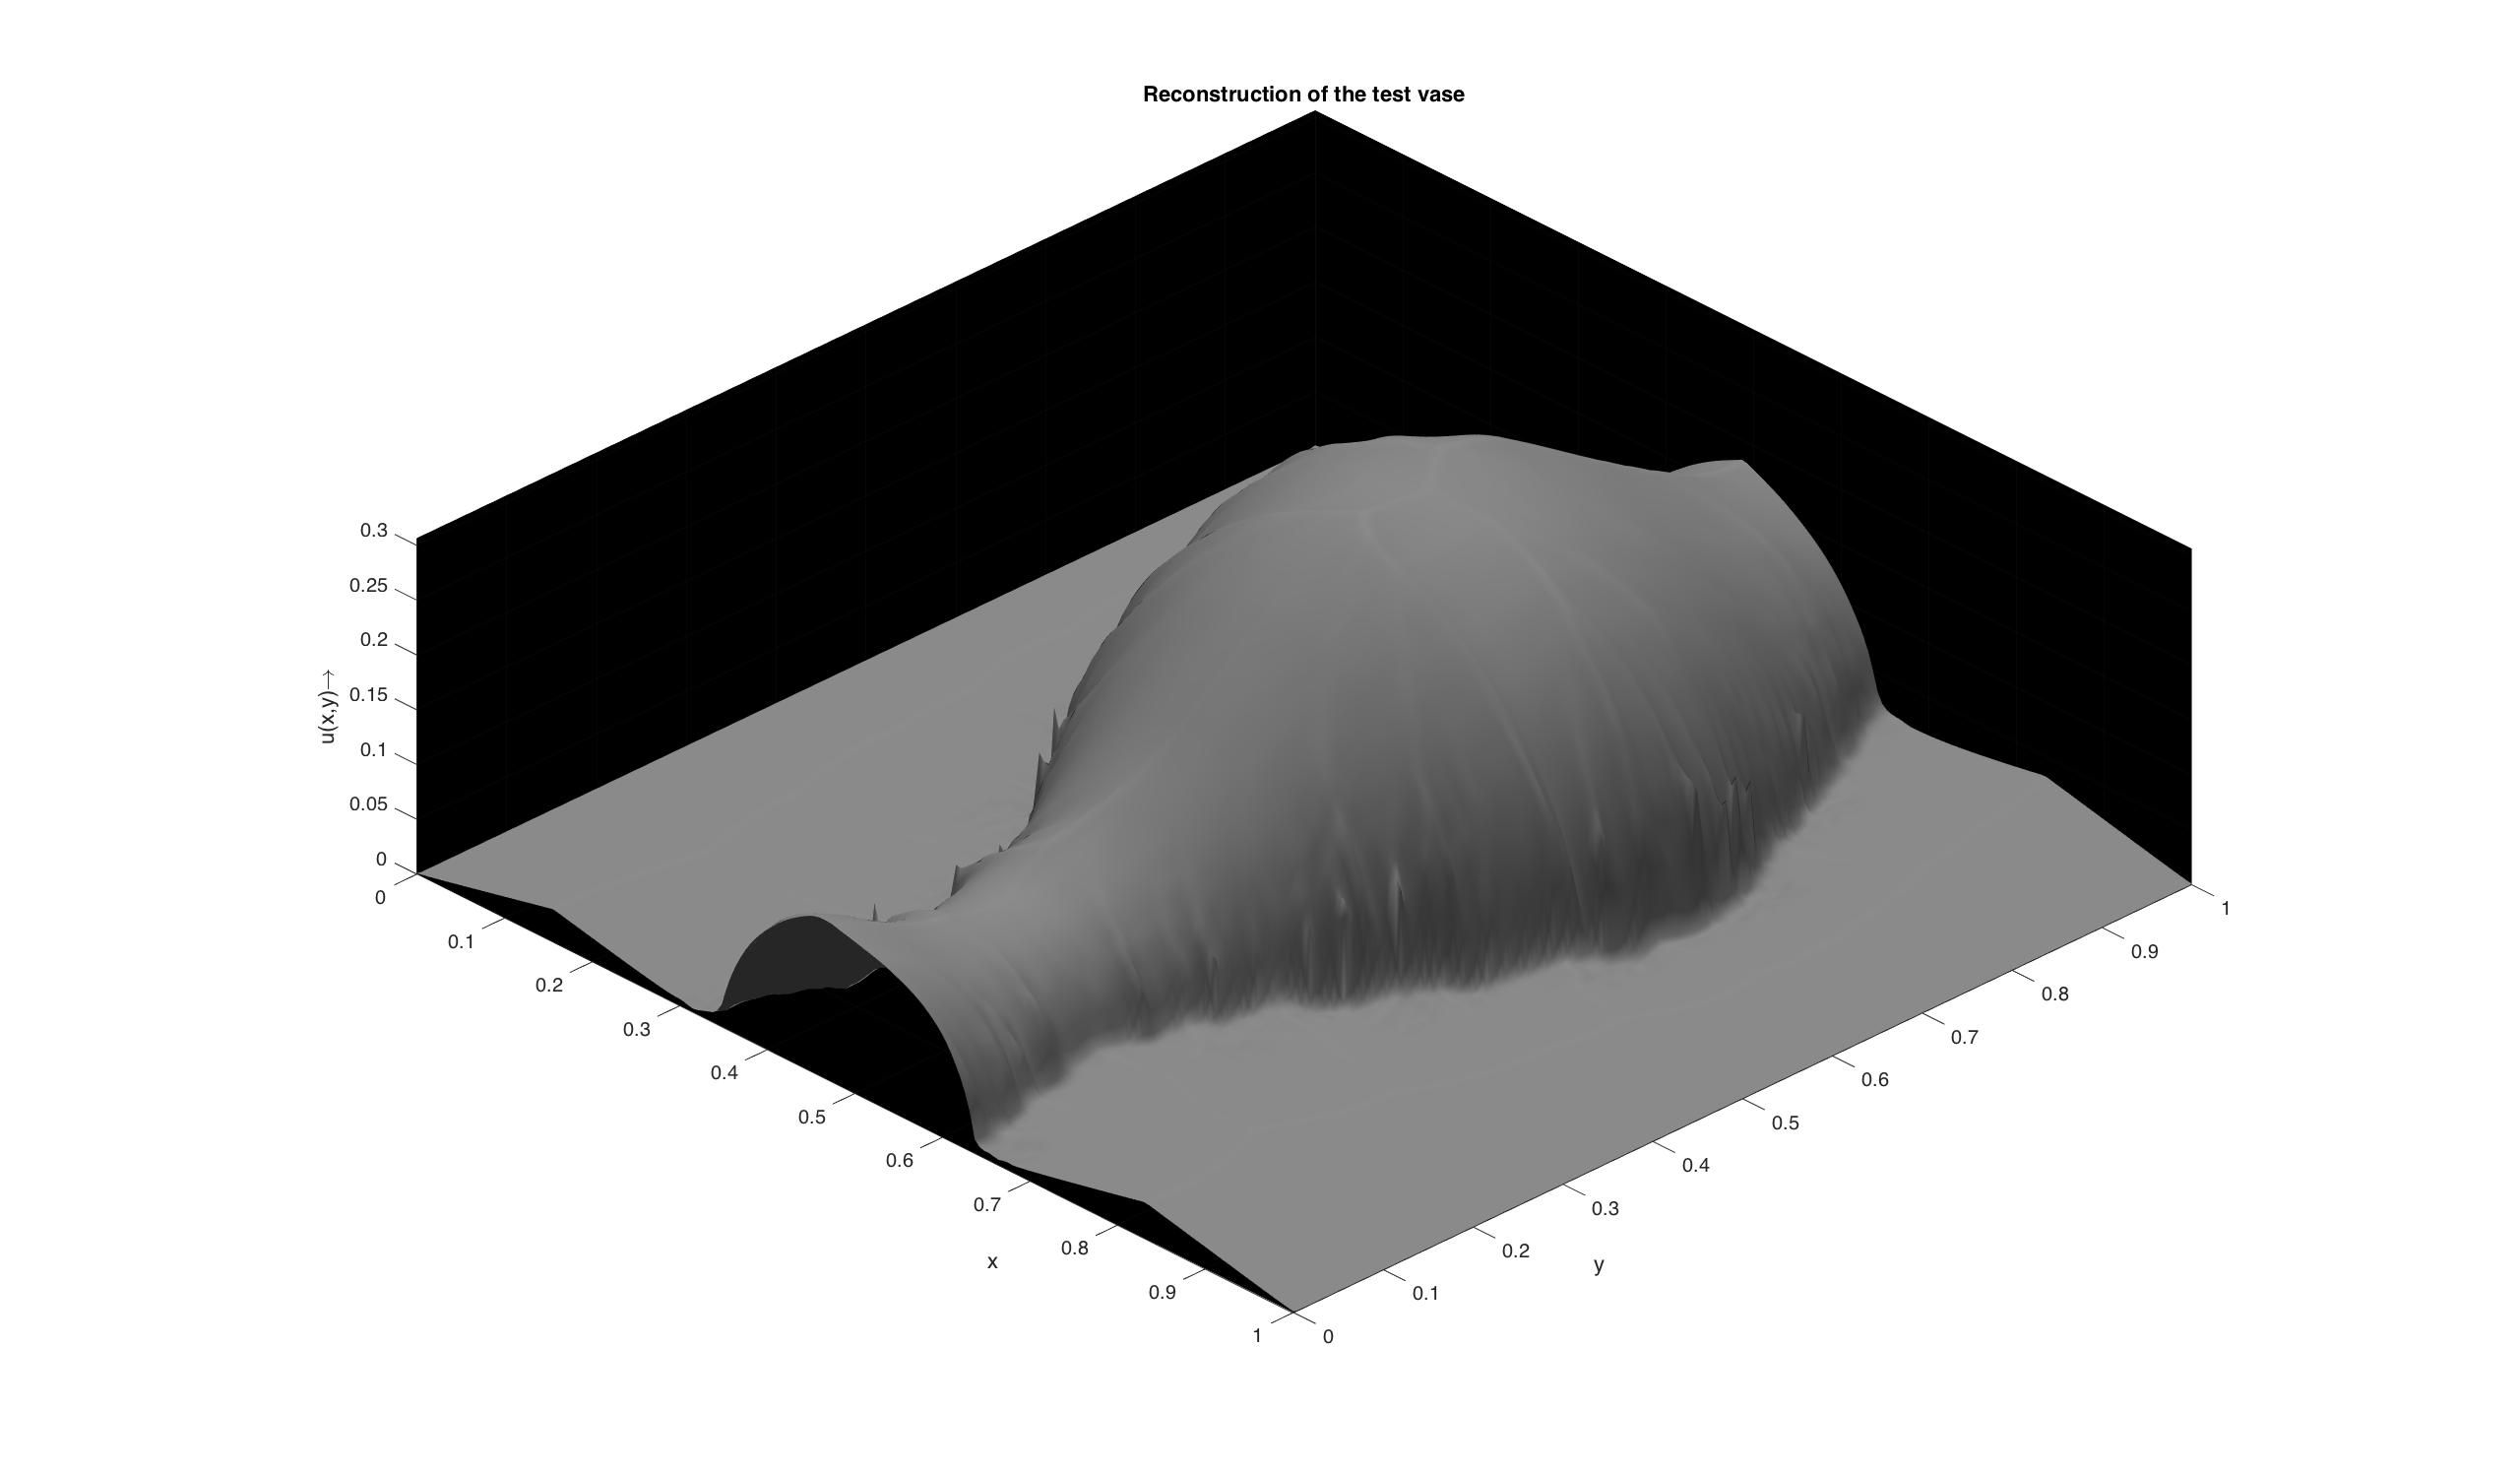
\includegraphics[scale = 0.15]{Images/vase.jpg}
	\caption{Reconstruction of the Synthetic Test Vase}
	\label{fig:15}
\end{figure}

\section{Perspective Projection Model}
The HJE\cite{prados2} governing the Perspective Projection Model is given by
\begin{eqnarray}
	-e^{-2v} + \frac{I(x)f^2}{Q(x)} \sqrt{f^2|\nabla v|^2 + (x.\nabla
		v)^2 + Q(x)^2} = 0 \qquad \text{in} \;\;\; \Omega
\end{eqnarray}

\noindent
We solve this equation by adding a transient $v_t$ term and then solve till we reach the steady state.
\begin{eqnarray}
v_t -e^{-2v} + \frac{I(x)f^2}{Q(x)} \sqrt{f^2|\nabla v|^2 + (x.\nabla
	v)^2 + Q(x)^2} = 0 \qquad \text{in} \;\;\; \Omega
\end{eqnarray} 

\noindent
To solve the time-dependent problem, we take the constant initial condition
\begin{equation}
	v_0 = -\frac{1}{2}\ln(\min_{x\in\Omega} I(x)f^2)
\end{equation}
to ensure convergence to the solution as discussed in Chapter 4. Refer \cite{prados2} for more details. We used the intensity image and attempted to reconstruct the original 3D shape. The input image along with the reconstructed images are shown in Figure (\ref{moz}). Steady State was taken to be $\lVert U^{n+1} - U^n \rVert < 10^{-16}$.
\begin{center}
	\begin{figure}
	\begin{subfigure}{0.5\textwidth}
		\centering
		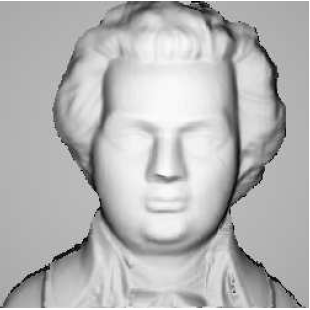
\includegraphics[scale = 0.85]{Images/moz.png}
		\caption{Intensity Image for Mozart}
	\end{subfigure}
	\begin{subfigure}{0.5\textwidth}
				\centering
				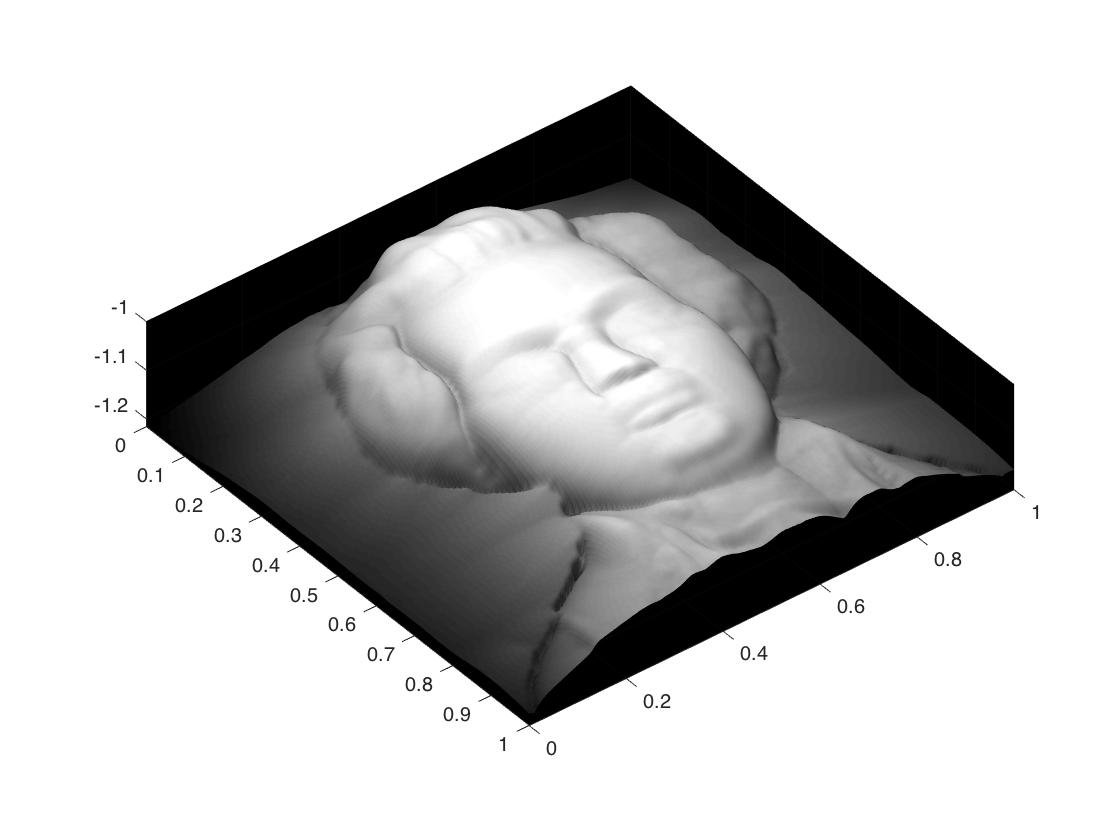
\includegraphics[scale = 0.24]{Images/moz.jpg}
				\caption{Reconstructed Face of Mozart}
	\end{subfigure}
		\begin{subfigure}{0.5\textwidth}
			\centering
			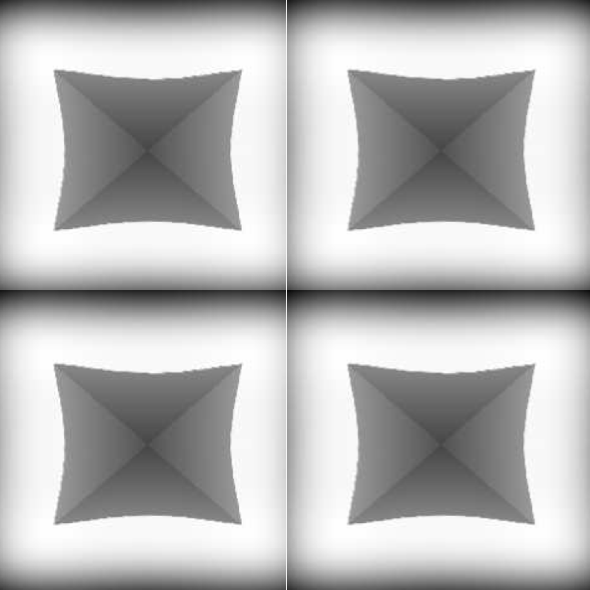
\includegraphics[scale = 0.5]{Images/thing4.png}
			\caption{Intensity Image for Test}
		\end{subfigure}
		\begin{subfigure}{0.5\textwidth}
			\centering
			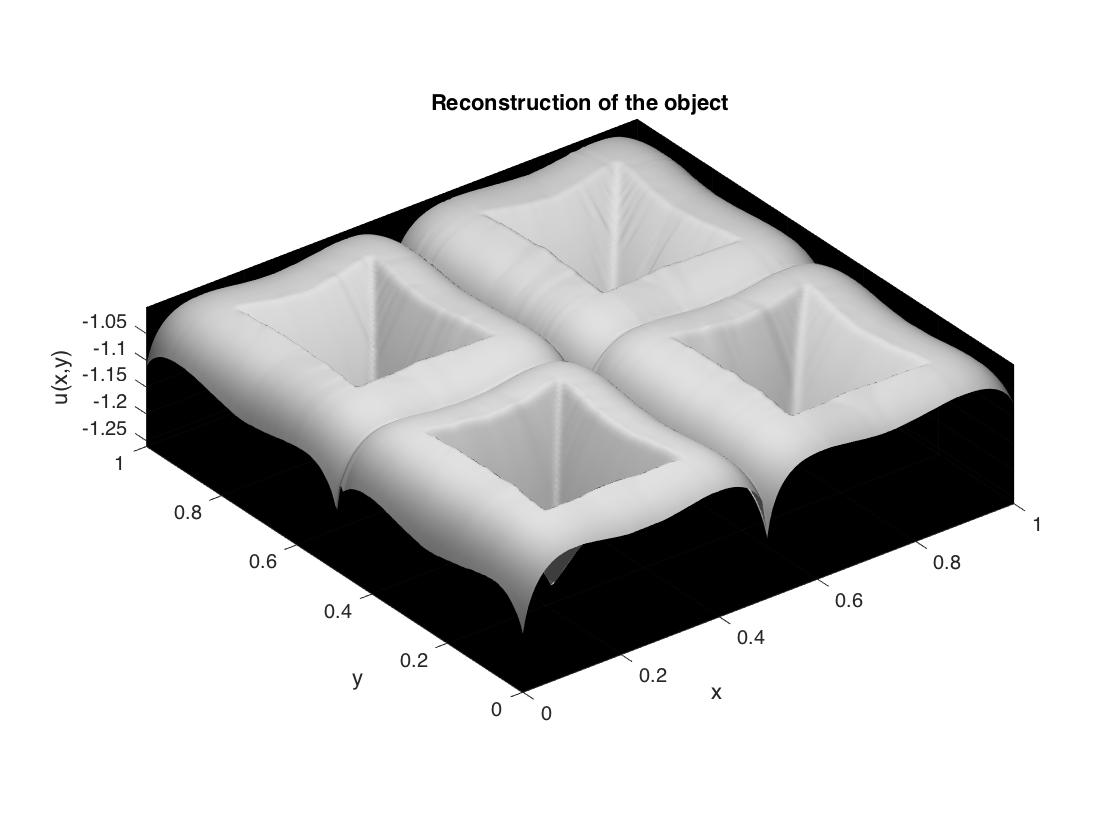
\includegraphics[scale = 0.24]{Images/thing4.jpg}
			\caption{Reconstructed Test Image}
		\end{subfigure}
	\caption{Reconstruction using Perspective Model by Prados \cite{prados2}}
	\label{moz}
\end{figure}
\end{center}
\noindent
The time evolution of the Mozart Face is shown in Figure (\ref{fig:evol}). 
\begin{center}
	\begin{figure}
		\begin{subfigure}{0.5\textwidth}
			\centering
			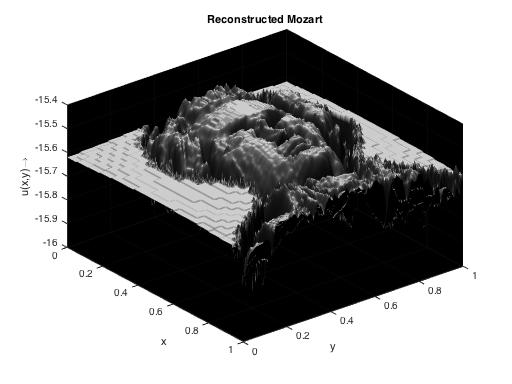
\includegraphics[scale = 0.4]{Images/moz/moz_100.jpg}
			\caption{100 Iterations}
		\end{subfigure}
		\begin{subfigure}{0.5\textwidth}
			\centering
			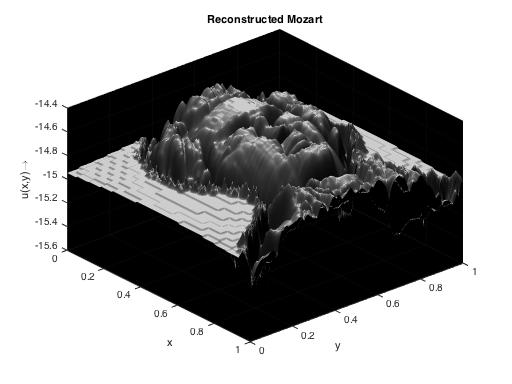
\includegraphics[scale = 0.4]{Images/moz/moz_300.jpg}
			\caption{300 Iterations}
		\end{subfigure}
		\begin{subfigure}{0.5\textwidth}
			\centering
			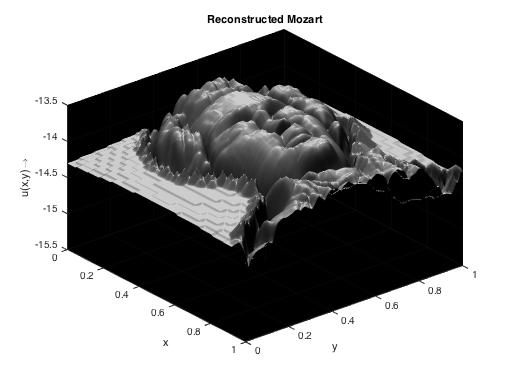
\includegraphics[scale = 0.4]{Images/moz/moz_500.jpg}
			\caption{500 Iterations}
		\end{subfigure}
		\begin{subfigure}{0.5\textwidth}
			\centering
			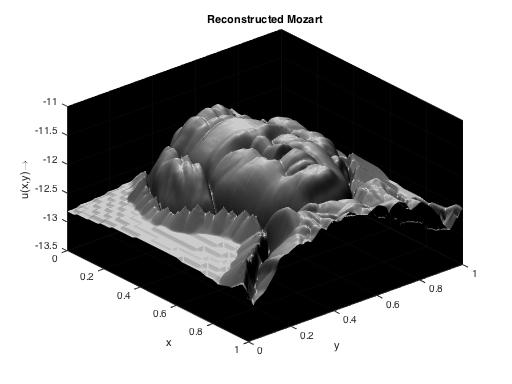
\includegraphics[scale = 0.4]{Images/moz/moz_1000.jpg}
			\caption{1000 Iterations}
		\end{subfigure}
		\begin{subfigure}{0.5\textwidth}
			\centering
			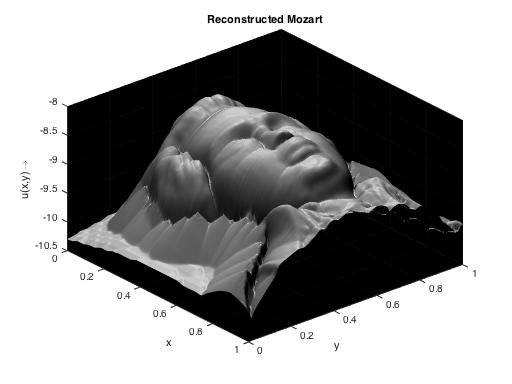
\includegraphics[scale = 0.4]{Images/moz/moz_2000.jpg}
			\caption{2000 Iterations}
		\end{subfigure}
		\begin{subfigure}{0.5\textwidth}
			\centering
			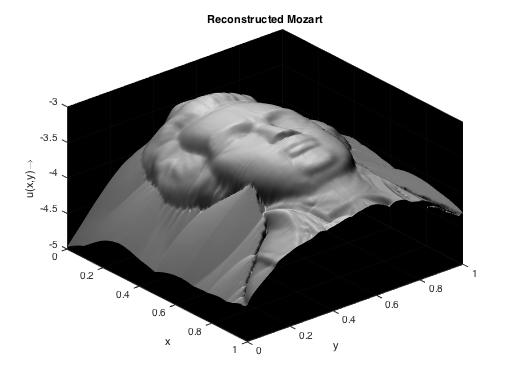
\includegraphics[scale = 0.4]{Images/moz/moz_5000.jpg}
			\caption{5000 Iterations}
		\end{subfigure}
		\caption{Time evolution of Mozart's Face}
		\label{fig:evol}
	\end{figure}
\end{center}

\noindent
\begin{center}
	\begin{figure}
		\begin{subfigure}{0.5\textwidth}
			\centering
			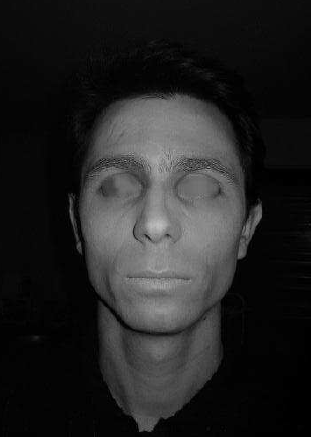
\includegraphics[scale = 0.35]{Images/realface/gleb_closed.png}
			\caption{Input Image for Real Face}
		\end{subfigure}
		\begin{subfigure}{0.5\textwidth}
			\centering
			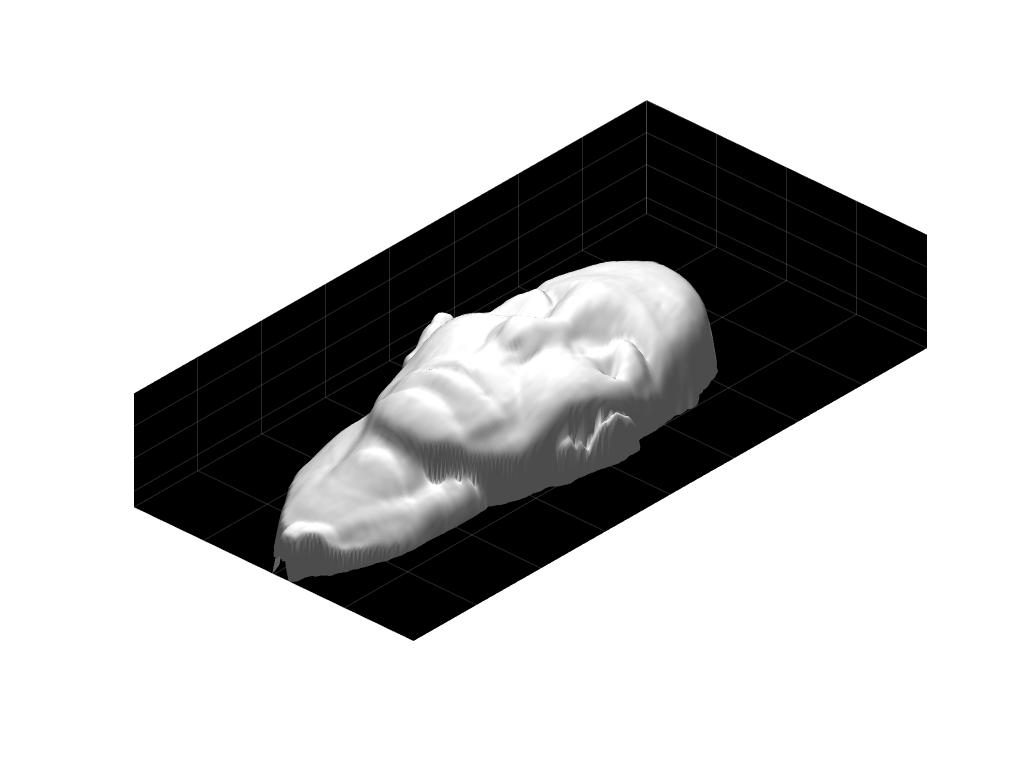
\includegraphics[scale = 0.2]{Images/realface/gleb_closed.jpg}
			\caption{Reconstructed}
		\end{subfigure}
		\begin{subfigure}{0.5\textwidth}
			\centering
			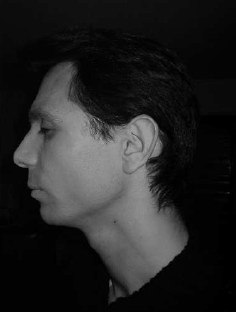
\includegraphics[scale = 0.902]{Images/realface/gleb_side.png}
			\caption{Input image for side view}
		\end{subfigure}
		\begin{subfigure}{0.5\textwidth}
			\centering
			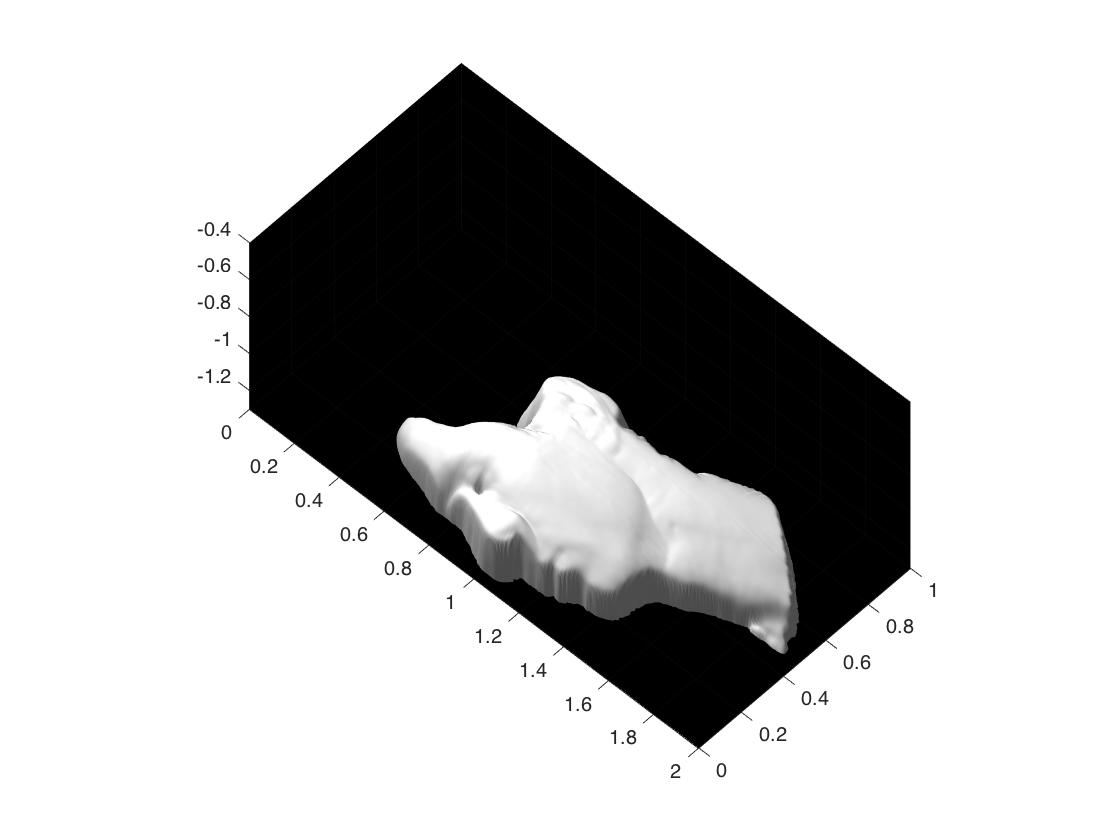
\includegraphics[scale = 0.2]{Images/realface/gleb_side.jpg}
			\caption{Reconstructed}
		\end{subfigure}
		\begin{subfigure}{0.5\textwidth}
			\centering
			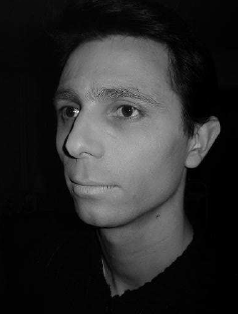
\includegraphics[scale = 0.902]{Images/realface/gleb_oblique.png}
			\caption{Input image for oblique view}
		\end{subfigure}
		\begin{subfigure}{0.5\textwidth}
			\centering
			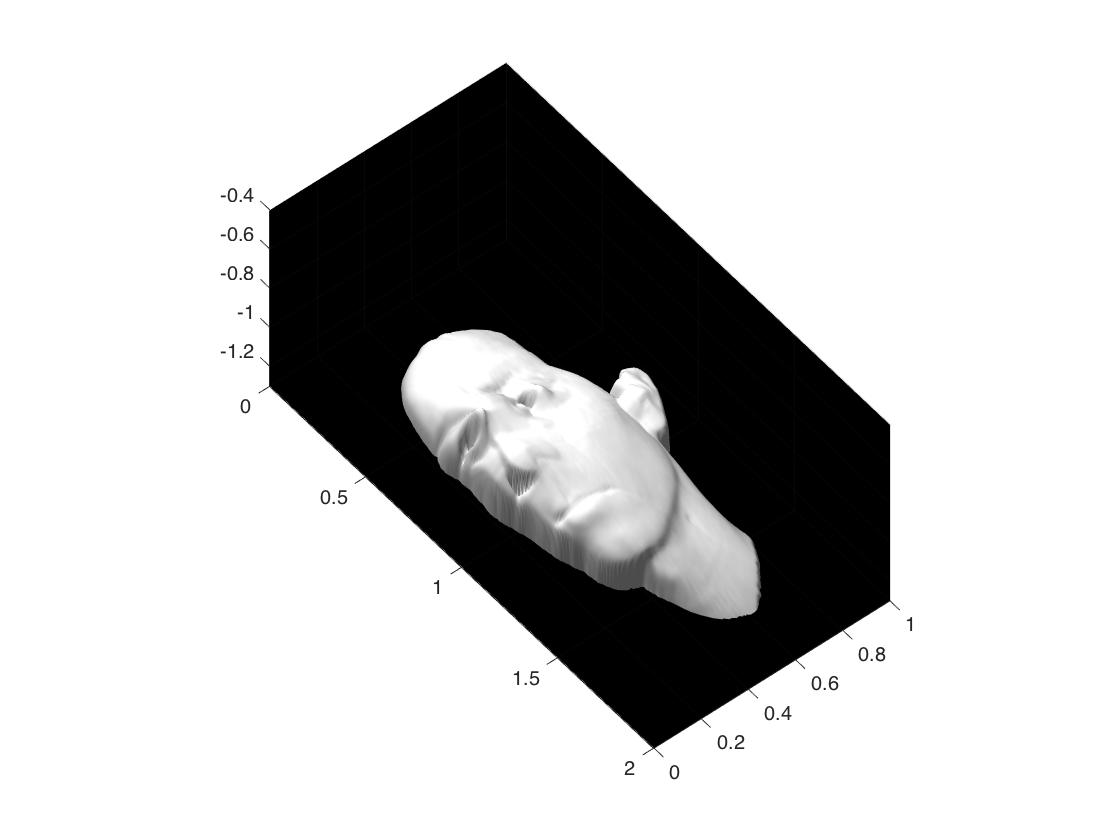
\includegraphics[scale = 0.2]{Images/realface/gleb_oblique.jpg}
			\caption{Reconstructed}
		\end{subfigure}
		\caption{Real Life Reconstructions}
		\label{fig:real}
	\end{figure}
\end{center}
 

	\chapter{Conclusion}
	So far in this report, we have explored Shape from Shading problems which focus on \emph{lambertian} surfaces, an assumption does not hold for real life objects except for a very few cases. Thus, these models cannot be used for real life applications extensively. But nonetheless SFS has innumerous applications viz. \emph{medical imaging, face reconstruction, terrain mapping, page reconstruction} and so on.\\
	
	\noindent 
	SFS is a simple yet a powerful tool for object reconstruction as it requires minimal input to reconstruct the original scene although the problem becomes difficult for complex cases. \\
	
	\noindent
	This work can be extended to accomodate the non-lambertian parameters to the Hamilton Jacobi equation in order to get closer to reality. On the other hand analysis namely, existence and uniqueness becomes difficult to study. Also regarding the numerics, one can attempt to develop higher order schemes to improve the accuracy of the solution.\\
	
	\noindent 
	Therefore, there is still room for improvements. It would be very nice if this work has
	inspired its readers to contribute to the related fields. \\
	
	\noindent
	For readers who wish to see the code that were used for reconstructions can visit.
	\begin{center}
		\href{https://www.github.com/Balaje/TIFR.git}{https://www.github.com/Balaje/TIFR.git}
	\end{center}
	
	\nocite{*}
	\bibliographystyle{acm}
	\bibliography{biblio}
\end{document}

%%% Local Variables:
%%% mode: latex
%%% TeX-master: "latexop.pdf"
%%% End:
